\documentclass[a5paper, 9pt, twoside]{book}

\usepackage[utf8]{inputenc}
\usepackage[ngerman]{babel}
\usepackage{extsizes}
\usepackage{natbib}
\usepackage{graphicx}
\usepackage[usenames,dvipsnames,svgnames,table]{xcolor}
\usepackage{wrapfig}
\usepackage[top=27mm, bottom=18mm, outer=15mm, inner=22mm]{geometry}
\usepackage{amsmath}
\usepackage{amssymb}
\usepackage{gensymb}
\usepackage{inconsolata}
\usepackage{url}
\usepackage{hyperref}
\usepackage{framed}
\usepackage{multicol}
\usepackage{tabto}
\usepackage{verbatim}
\usepackage{wrapfig}
%\usepackage{•}

\setcounter{tocdepth}{1}
\setcounter{secnumdepth}{2}
%\renewcommand{\thesection}{\arabic{section}}

%\righthyphenmin=2
%\lefthyphenmin=2
\sloppy

%\setlength{\parindent}{0pt}	% Hilfreich für Code --> keine Einrückung pro Paragraph
%\newcommand{\tab}{\hspace*{10mm}}
\newcommand{\version}{0.0.0.3 pre-alpha}
\newcommand{\referenz}[1]{Sektion \ref{#1} auf Seite \pageref{#1}: \nameref{#1}}
\newcommand{\gleichungsreferenz}[1]{Gleichung \ref{#1} auf Seite \pageref{#1}}
\newcommand{\casio}[1]{Casio fx-991xx: Konstante Nr. #1}
\hypersetup{colorlinks=true, linkcolor=NavyBlue}

\graphicspath{{Pictures/}}

\title{Physik Kompendium -- 11. Klasse bis zum Abitur}
\author{Till Blaha \& Leonard Geilen}

\begin{document}
\maketitle

\tableofcontents
\newpage

\chapter*{Vorwort}

\section*{Lizenz}

Die Autoren übernehmen keine Garantie, in welchem Zusammenhang auch immer, für die Richtigkeit oder Verständlichkeit dieses Dokuments. Es ist nur als Zusammenfassung und Unterstützung beim Lernen gedacht, nicht als alleiniges Lehrmaterial.

Dieses Dokument ist unter der \emph{GNU Free Documentation License}\footnote{Englischer Orginaltext liegt bei oder ist hier erhältlich: \url{https://www.gnu.org/licenses/fdl.txt}} lizenziert. Diese stellt es jedem frei, dieses Dokument unter gewissen Auflagen zu vertreiben oder zu ändern. Diese Auflagen beinhalten zum Beispiel, dass das weitervertriebene Produkt auch frei sein muss und dass bei einer Änderung des Dokumentes der Name des Autors und ein Beschreibung der Änderung beigefügt werden muss. Für genauere Details ziehen Sie bitte den originalen Lizenztext heran.

Für die Bereitstellung des \LaTeX{} Quellcodes zum Ändern oä. bitte ich, mich per Email direkt zu kontaktieren.

Die Autoren sind außerdem für jegliche Meinungen, Korrekturen, Anregungen und wüste Beschimpfungen offen:

\href{mailto:till.blaha@web.de}{till.blaha@web.de}


\section*{Umfang}

Dieses Material basiert auf dem Umfang des \glqq Regionalcurriculum für das Fach Physik, Prüfungsregion 12\grqq .\footnote{Orginaltext: \url{http://www.idsb.eu/intranet/teamworks.dll/Internal/document/0xD4A9A3187641B24EB79D9320B3060289/SC-RC\%20Physik\%2010-12.pdf}}


\section*{Version}

Bei diesem Dokument handelt es sich um die Version \version , kompiliert am \today . Aufgrund vieler formaler und inhaltlicher Fehler sowie Unvollständigkeit, nicht für die Veröffentlichung bestimmt.


\chapter{Elektrisches Feld}
\section{Beweis für die Existenz}

%%%%% Elektrisches Feld %%%%%
%% #1 Beweis %%


%Some sample text to be displayed above the first subsection

%\subsection{Prinzip}

%Ein Zyklotron besteht aus Zwei hohlen, halbzylindrischen und Duanden an denen eine Spannung mit unterschiedlichem Vorzeichen anliegt, und darüber bzw. darunter liegende Magneten, die ein homogenes Magnetfeld erzeugen. Zudem gibt es einen Einlass und einen Auslass für Teilchen.

%\begin{wrapfigure}{r}{0.4\textwidth} \label{Zyklo}
%
%	\vspace{-10pt}
%	\includegraphics[width=0.35\textwidth]{Zyklotron_Prinzipskizze02.png}
%	\vspace{-13pt}
%	\caption{Prinzipskizze eines Zyklotrons}
%	\vspace{-5pt}	
%	
%\end{wrapfigure}

%\subsubsection{Anwendung}

% Some Formula:

%\begin{equation}
%	x= \frac{y \cdot 13 \pi z}
%			{\cos \alpha}
%\end{equation}

%%%%%%%%%%%%%%%%%%%%%%%
% Eigentlicher Beginn %
%%%%%%%%%%%%%%%%%%%%%%%

\subsection{Elektrostatik}

Wenn ein Körper geladen ist, bedeutet das, dass positive und negative Ladungen in ungleich große Mengen vorhanden sind. Daraus folgt, dass sich gleichgroße Mengen ungleichnamiger (positiv $\neq$ negativ) Ladungen neutralisieren.

Gleichnamige Landungen stoßen sich ab, während ungleichnamige Ladung sich anziehen. Dies ähnelt sehr dem magnetischen Feld und steht den Gravitationsfeldern entgegen, die sich ausschließlich gegenseitig anziehen.

In Metallen sind die negativen Ladungen beweglich, sie heißen Elektronen. Diese Eigenschaft macht Metalle zu \glqq Leitern\grqq .

\begin{leftbar}
Nice to know: der Begriff Elektron (und alles davon abgeleitete Begriffe) kommt vom altgriechischen Wort \glqq élektron\grqq{} und bedeutet \glqq Bernstein\grqq . Den Effekt der Ladung wurde schon im alten Griechenland an Bernstein entdeckt.
\end{leftbar}


\subsection{Elektroskop}

Ein Elektroskop besteht aus einer Schnecke aus Metallband. Ein Zeiger, der sich an der Schnecke befindet, schlägt aus, sobald es einen Überschuss an positiver oder negativer Ladung gibt, da sich dann durch die gleichnamige Ladungen die vielen Windungen gegenseitig voneinander Abstoßen.

\subsection{Influenz} \label{subsec:Influenz}

Nun ist es logisch, dass bei Berührung eines Elektroskops mit einem negativ geladenen Körper, die Nadel ausschlägt, da das Metallband diese Elektronen leitet und ein Überschuss an negativer Ladung in der Schnecke zum Ausschlag führt.

Aber auch wenn ein beliebig geladener Körper (beispielsweise ein positiv geladener Kunststoffstab) nur über das Elektroskop gehalten wird, ohne es zu berühren, schlägt die Nadel aus. Dies nennt man \emph{Influenz} und das Phänomen beruht darauf, dass sich ungleichnamige Ladungen anziehen. Die beweglichen negativen Ladungen wandern durch die Anziehung des positiven Kunststoffstabs weg von der Schnecke und hinterlassen einen Überschuss an positiven Ladungen, sodass die Nadel ausschlägt. Entfernt man den Stab wieder, gelangt der Zeiger wieder in die Ausgangslage.

Das Besondere dabei ist, dass diese Influenz kein Medium benötigt, also auch im Vakuum über Distanzen auftritt. Damit ist ein Feldcharakter bewiesen.




\section{Modellierung und Mathematisierung}

%%%%% Elektrisches Feld %%%%%
%% #2 Modellierung und Mathematisierung %%


%Some sample text to be displayed above the first subsection

%\subsection{Prinzip}

%Ein Zyklotron besteht aus Zwei hohlen, halbzylindrischen und Duanden an denen eine Spannung mit unterschiedlichem Vorzeichen anliegt, und darüber bzw. darunter liegende Magneten, die ein homogenes Magnetfeld erzeugen. Zudem gibt es einen Einlass und einen Auslass für Teilchen.

%\begin{wrapfigure}{r}{0.4\textwidth} \label{Zyklo}
%
%	\vspace{-10pt}
%	\includegraphics[width=0.35\textwidth]{Zyklotron_Prinzipskizze02.png}
%	\vspace{-13pt}
%	\caption{Prinzipskizze eines Zyklotrons}
%	\vspace{-5pt}	
%	
%\end{wrapfigure}

%\subsubsection{Anwendung}

% Some Formula:

%\begin{equation}
%	x= \frac{y \cdot 13 \pi z}
%			{\cos \alpha}
%\end{equation}

%%%%%%%%%%%%%%%%%%%%%%%
% Eigentlicher Beginn %
%%%%%%%%%%%%%%%%%%%%%%%

Um das Phänomen der Influenz und vieles Weitere rund um die Elektrizität zu beschreiben, wurde das Modell des Elektrischen entwickelt. 

\begin{NiceToKnow}
Generell geht es in der Physik nicht unbedingt darum, zu erläutern, wie etwas genau funktioniert, da vieles, wie zum Beispiel die eigentliche Beschaffenheit von Feldern, (noch) gar nicht genau zu erklären ist. Es geht darum, Modelle zu entwickeln, mit deren Hilfe sich mathematische Ausdrücke zur Beschreibung von diesen Phänomenen ableiten lassen.
\end{NiceToKnow}


\subsection{Feldlinien}

\begin{figure}
	\centering
	\includegraphics[width=0.6\textwidth]{EFeld}
	\caption{Feldlinien zwischen zwei geladenen Teilchen}
\end{figure}

Feldlinien\footnote{Abbildung von: \url{https://elearning.physik.uni-frankfurt.de/data/FB13-PhysikOnline/lm_data/lm_282/auto/kap16/picts/epm.gif}} sind ein Modell zur Verdeutlichung von grundlegenden Eigenschaften eines elektrischen Feldes. Sie schneiden sich nie und haben eine Richtung, die durch Pfeile angezeigt wird. Sollten sie von einem Körper ausgehen oder auf einen Körper auftreffen, stehen sie senkrecht auf dessen Oberfläche. Außerdem gibt die Dichte der Linien die Stärke des Feldes an.\footnote{Armin Kunz: Bewertung der 1. Klausur vom 09.10.2014} Die Pfeile der Feldlinien zeigen immer zur negativen Ladung.


\subsection{Coulomb'sches Gesetz} \label{subsec:CoulombGesetz}

Wenn nun gesetzt ist, dass sich Ladungen beeinflussen, ist der nächste Schritt diesen \glqq Einfluss\grqq{} mathematisch auszudrücken. Dazu gibt es das Coulomb'sche Gesetz, welches die Kraft die zwei kugenförmige (sphärische) Körper aufeinander auswirken, in Abhängigkeit von deren Ladungen und dem Abstand angibt:

\begin{equation} \label{eq:coulomb_gesetz}
	F = \frac{1}{4\pi \cdot \epsilon_0} \cdot \frac{Q_1 \cdot Q_2}{d^{2}}
\end{equation}

Die Gleichung besteht aus einem konstanten Faktor, der die sogenannte \glqq elektrische Feldkonstante\grqq{} $\epsilon_0$ beinhaltet (\casio{32}), und einem variablen Teil der die Beträge der beiden Ladungen $Q_1$ und $Q_2$, und den Abstand der Mittelpunkte $d$ enthält.

Die Einheit Ladung ist $C$ (sprich: Coulomb), was gleich $A \cdot s$ ist. Eine Einheitenrechnung sieht dann wie folgt aus:

\begin{align}\label{eq:coulomb_gesetz_einheiten}
\begin{split}
	N 							&= \frac{1}{\epsilon_0} \cdot \frac{As \cdot As}{m^{2}} \\
	\frac{kg \cdot m}{s^{2}} 	&= \frac{1}{\epsilon_0} \cdot \frac{A^{2} \cdot s^{2}}{m^{2}}
\end{split}
\end{align}

Daraus ergibt sich als Einheit für die Feldkonstante $\epsilon_0$:

\begin{align}\label{eq:feldkonstante_einheiten}
\begin{split}
	\epsilon_0 &= \frac{A^{2} \cdot s^{2}}{m^{2}} \cdot \frac{s^{2}}{kg \cdot m} \\
	\epsilon_0 &= \frac{A^{2} \cdot s^{4}}{m^{3} \cdot kg} \\
	\epsilon_0 &= \frac{As}{Vm}
\end{split}
\end{align}

\begin{Aufgabe}
Versuche über die Definition des Volts ($V=\frac{kg \cdot m^2}{A \cdot s^3}$) von der vorletzten auf die letzte Umformung zu kommen!
\end{Aufgabe}

\begin{NiceToKnow}
Diese Form der Gleichung ist analog zu Newtons Gravitationsgesetz: $F = G \cdot \frac{m_1 \cdot m_2}{d^2}$. Hierbei ist $G$ ebenfalls eine Konstante, nämlich die Gravitätskonstante.
\end{NiceToKnow}


\subsection{Feldstärke}  \label{subsec:Feldstaerke}

In einem homogenen Feld ist die Feldstärke (Formelzeichen: $E$) also an jedem Punkt gleich. Sie ordnet jedem geladenen Körper eine Kraft und, sollte mit Vektoren gerechnet werden, eine Richtung zu:

\begin{equation} \label{eq:feldstaerke}
	\vec{E} = \frac{\vec{F}}{q}
\end{equation}

\noindent $q$ ist hierbei die \emph{vorzeichenbehaftete} Ladung des Probekörpers im Feld. Als Einheit ergibt sich $\frac{N}{C}$ für die Feldstärke $E$. 

Umgeformt für $F$ ergibt sich aus der Gleichung:

\begin{equation} \label{eq:feldstaerke_nach_F}
	\vec{F} = q \cdot \vec{E}
\end{equation}


\subsection{Homogenes Feld} \label{subsec:EFeldHomogen}

Das elektrische Feld zwischen zwei geladenen Körpern ist meistens inhomogen. Das heißt, dass die Feldstärke, also die Dichte der Feldlinien nicht überall gleich ist. Für Berechnungen würde dies das Lösen von komplexen Differentialgleichungen voraussetzen. Daher wird in der Schulphysik fast immer von einem homogenen Feld ausgegangen, wenn Berechnungen an einem elektrischen Feld anstehen:

\begin{itemize}
	\item Die Feldlinien zeigen alle in dieselbe Richtung
	\item Die Feldlinien haben alle denselben Abstand zueinander
\end{itemize} 

Eine Möglichkeit, so ein Feld zu generieren, ist der Plattenkondensator (\referenz{sec:plattenkondensator}).








\section{Phänomene}

Im Folgenden werden bei der Nennung von \glqq Wellen\grqq{} immer Transversalwellen gemeint, wenn es keine weitere Anmerkung gibt.  


\subsection[Ausbreitung in Elementarwellen]{Ausbreitung in Elementarwellen (Huygens'sches Prinzip)} \label{subsec:ausbreitung}

Das Huygens'sche Prinzip macht eine wichtige Aussage zur Ausbreitung von Wellen:

\glqq Jedes Teilchen (Oszillator), das von einer Wellenfront erfasst wird, löst von sich aus eine zirkulare Welle nach allen Seiten aus.\grqq{} Die eigentlich sichtbare Wellenfront ist nach Huygens eine Einhüllende aller \glqq Elementarwellen\grqq . Dadurch ist es Wellen unter anderem möglich in den geometrischen Schattenraum zu propagieren. \referenz{subsec:doppelspalt}


\subsection{Reflexion}  \label{subsec:Reflexion}

	\subsubsection{Fixiertes Ende}
	
	Wenn eine Welle von einem fixierten Ende (eingespannt) reflektiert wird, dann gibt es einen Phasensprung von $180 \degree$ oder $\pi$, bzw $\frac{\lambda}{2}$.
	
	\subsubsection{Loses Ende}
	
	Trifft eine Welle auf ein loses Ende, dann wird sie ohne Phasensprung reflektiert.



\subsection{Überlagerung} \label{subsec:ueberlagerung}

Wenn sich Wellen in einem räumlichen Punkt treffen, dann überlagern sie sich und bilden eine summierte Welle. Wenn also ein Wellenberg auf einen Wellenberg trifft, addieren sich beide Welle und der resultierende Wellenberg ist höher. Sollte auf einen Wellenberg ein Wellental treffen wird auf addiert, und die resultierende Welle von der Amplitude her kleiner.

Nachdem sich die Wellen in diesem Punkt überlagert haben, laufen beide weiter ohne die andere zu beeinflussen; so als hätte es die Überlagerung nie gegeben.

	\subsubsection{Stehende Welle}
	
	Wenn sich gegenläufige, das heißt parallel und identisch, aber in die entgegengesetzte Richtung fortschreitende, Wellen mit derselben Wellenlänge überlagern, entsteht eine stehende Welle. 
	Das heißt, dass es mindestens 2 Oszillatoren auf dieser Welle gibt, die sich gar nicht bewegen (\glqq stehen\grqq), die sogenannten Knotenpunkte.
	
	Eine stehende Welle kann zum Beispiel ausgelöst werden, wenn bei einer Reflexion am festen Ende die Hälfte der Wellenlänge $\lambda$ ein ganzzahliges Vielfaches der Abstands $l$ der beiden Enden ist. $k$ ist in diesem Fall eine Variable, die nur positive ganze Zahlen annehmen kann:
	
	\begin{equation} \label{stehendewelle}
		\lambda = 2k \cdot l \quad wobei \ k \in 1,2,3...
	\end{equation}



\subsection{Interferenzen} \label{sec:interferenz}
%cue for pic
Wenn sich Wellen, die nicht nur dieselbe Wellenlänge, sondern auch die selbe Amplitude aufweisen, in einem Punkt überlagern, dann kann es zu Interferenzen kommen.

	\subsubsection{Konstruktive Interferenz}
	
	Wenn in dem Punkt beide Wellen ein Maximum aufweisen, sich also zu einem höheren Wellenberg addieren, spricht man von konstruktiver Interferenz.
	
	Dazu muss der Gangunterschied $\delta$ ein ganzzahliges Vielfaches der Wellenlänge sein:
	
	\begin{equation}	\label{eq:kon_interferenz}
		\delta = k \cdot \lambda \ \ \ wobei \ \ k \in 1,2,3...
	\end{equation}
	
	\subsubsection{Destruktive Interferenz}
	
	Im Gegensatz zur konstruktiven Interferenz, treffen nun also Wellen aufeinander, die einmal einen Wellenberg und einmal ein Wellental aufweisen. Da sie dieselbe Amplitude haben, ist die resultierende Amplitude im betroffenen Punkt $0$.
	
	Der Gangunterschied $\delta$ muss daher die Summe eines ganzzahliges Vielfaches Wellenlänge und der halben Wellenlänge sein:
	
	\begin{equation}
		\delta = k \cdot \lambda + \frac{\lambda}{2} \ \ \ wobei \ \ k \in 1,2,3...
	\end{equation}

	Zur einfacheren Umstellung nach $\lambda$ existiert diese, internationale Form:
	
	\begin{equation} \label{eq:des_interferenz}
		\delta = (2k -1) \cdot \frac{\lambda}{2} \ \ \ wobei \ \ k \in 1,2,3...
	\end{equation}


\section{Plattenkondensator} \label{sec:plattenkondensator}

%%%%% Elektrisches Feld %%%%%
%% #3 Kondensator %%


%Some sample text to be displayed above the first subsection

%\subsection{Prinzip}

%Ein Zyklotron besteht aus Zwei hohlen, halbzylindrischen und Duanden an denen eine Spannung mit unterschiedlichem Vorzeichen anliegt, und darüber bzw. darunter liegende Magneten, die ein homogenes Magnetfeld erzeugen. Zudem gibt es einen Einlass und einen Auslass für Teilchen.

%\begin{wrapfigure}{r}{0.4\textwidth} \label{Zyklo}
%
%	\vspace{-10pt}
%	\includegraphics[width=0.35\textwidth]{Zyklotron_Prinzipskizze02.png}
%	\vspace{-13pt}
%	\caption{Prinzipskizze eines Zyklotrons}
%	\vspace{-5pt}	
%	
%\end{wrapfigure}

%\subsubsection{Anwendung}

% Some Formula:

%\begin{equation}
%	x= \frac{y \cdot 13 \pi z}
%			{\cos \alpha}
%\end{equation}

%%%%%%%%%%%%%%%%%%%%%%%
% Eigentlicher Beginn %
%%%%%%%%%%%%%%%%%%%%%%%

Der Plattenkondensator (im Folgenden nur noch Kondensator genannt) ist ein wichtiges Element der Elektrotechnik. Auch eignet er sich ebenfalls seht gut, um in der Schulphysik verschiedene Aspekte von elektrischen Feldern zu zeigen.


\subsection{Definition} \label{subsec:kon_def}

\begin{figure}[h!]
	\centering
	\includegraphics[width=0.6\textwidth]{RCWiring}
	\caption{Ein Schaltkreis mit Kondensator $C$ und Widerstand $R$}
	\label{fig:CapWirering}
\end{figure}

Ein Plattenkondensator besteht aus zwei ungleichnamig geladenen Platten, die sich parallel gegenüberstehen. Sie sind an ein Spannungsquelle angeschlossen. In einem Schaltplan wird er wie in Abbildung \ref{fig:CapWirering}\footnote{"RC switch" by PureCore - Own work. Licensed under CC BY-SA 3.0 via Commons - \url{https://commons.wikimedia.org/wiki/File:RC_switch.svg}} notiert.

\begin{leftbar}
Wichtig: An sich fließt kein Strom durch den Kondensator! Die Platten sind elektrisch getrennt; das Dielektrikum, also das nicht-leitende Material zwischen den Platten (z.B. Luft), isoliert. 
\end{leftbar}


\subsection{Elektrisches Feld im Inneren des Kondensators}

\begin{figure}[h!]
	\centering
	\includegraphics[width=0.8\textwidth]{EFeldKondensator}
	\caption{Das elektrische Feld in und um einen Plattenkondensator}
\end{figure}

Durch den Überschuss  positiver Ladungen auf der einen Seite und negativer Ladungen auf der Anderen ergibt sich ein homogenes Magnetfeld zwischen den Platten. \footnote{„E Feld Kondensator“. Über Wikibooks - \url{https://de.wikibooks.org/wiki/Datei:E_Feld_Kondensator.png}}

\subsubsection{Feldstärke}

Die Stärke des Feldes im Inneren lassen sich auf recht einfach Art aus der anliegenden Spannung $U$ und dem Plattenabstand $d$ berechnen:

\begin{equation} \label{eq:feldstaerke_kondensator}
	E = \frac{U}{d}
\end{equation}

Die resultierende Einheit $\frac{V}{m}$ ist äquivalent zu $\frac{N}{C}$.

\subsubsection{Kraft auf Körper}

In die allgemeine Gleichung für eine Kraft auf einen geladenen Körpern (Gleichung \ref{eq:feldstaerke_nach_F} auf Seite \pageref{eq:feldstaerke_nach_F}: $\vec{F} = q \cdot \vec{E}$) kann nun die obige Gleichung für $E$ im Kondensator eingesetzt werden (Gleichung \ref{eq:feldstaerke_kondensator} auf Seite \pageref{eq:feldstaerke_kondensator}):

\begin{equation} \label{eq:kraft_kondensator}
	F = q \cdot \frac{U}{d}
\end{equation}

In diesem Fall kann sowieso auf eine Vektorrechnung verzichtet werden, da die Richtung der des elektrischen Felds klar und homogen ist.

\subsubsection{Energieumsatz bei einer Bewegung eines Körpers}

Wenn ein Körper in einem Kondensator bewegt wird, wird dabei Energie umgesetzt. Ein äquivalente Ausdrucksweise wäre, es wird Arbeit verrichtet. Das geschieht gemäß dieser Formel, bei der $s$ die Strecke ist, um die der Körper verschoben wird:

\begin{equation} \label{eq:arbeit_kondensator}
	W = F \cdot s
\end{equation}

Die Kraft $F$ kann durch Umstellen mit $F = q \cdot \frac{U}{d}$ zu

\begin{equation} \label{eq:arbeit_kondensator_ersetzt}
	W = q \cdot E \cdot s
\end{equation}

ersetzt werden.

\begin{leftbar}
Nice to know: $W = q \cdot E \cdot s$ ist analog zur Lagearbeit aus der Mechanik: $W_{pot} = m \cdot g \cdot h$
\end{leftbar}


\subsection{Elektrische Feldstärke über die Flächenladungsdichte}

Die elektrische Feldstärke im Inneren eines Kondensators lässt sich auch über die Flächenladungsdichte berechnen. Die Flächenladungs\-dichte ($\sigma$) gibt an, wie dicht Ladungen auf den Kondensatorplatten verteilt sind:

\begin{equation} \label{eq:flaechenladungsdichte}
	\sigma = \frac{Q}{A}
\end{equation}

\begin{leftbar}
Nice to know: man schreibt $q$ für die spezifische, unveränderbare Ladung eines Probekörpers und $Q$ für z.B. die Ladung von Kondensatorplatten.
\end{leftbar}

Die Flächenladungsdichte ist im homogenen Feld proportional zur Feldstärke ($\sigma \sim E$). Die Proportionalitätskonstante hierbei ist $\frac{1}{\epsilon_0}$, sodass sich ergibt:

\begin{equation} \label{eq:feldstaerke_mit_sigma}
	E = \frac{\sigma}{\epsilon_0} = \frac{1}{\epsilon_0} \cdot \frac{Q}{A}
\end{equation}

\subsubsection{Flächenladungsdichte bei Kugeln}

Die Oberfläche von Kugeln ist als $A=4\pi \cdot r^2$ definiert. Daher ergibt sich der Spezialfall für die Feldstärke:

\begin{equation} \label{eq:feldstaerke_kugel}
	E = \frac{1}{\epsilon_0} \cdot \frac{Q}{4\pi \cdot r^2} = \frac{1}{4\pi \cdot \epsilon_0} \cdot \frac{Q}{r^2}
\end{equation}


\subsection{Kapazität des Kondensators}

Ein Kondensator lässt sich über seine Kapazität beschreiben:

\begin{equation}
	C = \frac{Q}{U}
\end{equation}

Die Kapazität gibt also an, wie viel Ladung ein Kondensator bei einer definierten Spannung fassen kann. Bzw. wie hoch die Spannung sein muss, damit die definierte Ladung $Q$ \glqq auf den Kondensator passt\grqq .

Für eine Bestimmungsgleichung, welche nur aus Kenngrößen besteht, muss Q ersetzt werden. Mit $E = \frac{\sigma}{\epsilon_0} <=> \frac{U}{d} = \frac{Q}{A \cdot \epsilon_0} <=> Q = \epsilon_0 \cdot \frac{U \cdot A}{d}$ kann man also auch schreiben:

\begin{equation}
	C = \epsilon_0 \epsilon_r \cdot \frac{U \cdot A}{d \cdot U} = \epsilon_0 \epsilon_r \cdot \frac{A}{d}
\end{equation}

Die Spannung $U$ kürzt sich und es wurde die relative Feldkonstante $\epsilon_r$ eingeführt, welche das Dielektrikum (\referenz{subsec:kon_def}) charakterisiert. Für Luft bzw. Vakuum ist sie $\approx 1$. Es gibt jedoch Materialien, die durch eine hohe relative Feldkonstante die Kapazität um hohe Faktoren erhöhen.

\begin{leftbar}
Nice to know: $BaTiO_3$, Bariumthiooxid, hat eine $\epsilon_r$ von $10^2-10^3$\footnote{Aus: \href{http://www.techniklexikon.net/d/dielektrizitaetskonstante/dielektrizitaetskonstante.htm}{http://www.techniklexikon.net/d/dielektrizitaetskonstante/\\ dielektrizitaetskonstante.htm}}
\end{leftbar}


\subsection{Verschaltung von Kondensatoren}

\subsubsection{Parallel}

\begin{figure}[h!]
	\centering
	\includegraphics[width=0.5\textwidth]{CapsParallel}
	\caption{Parallelschaltung zweier Kapazitiven (= Kondensatoren) $C_1$ und $C_2$}
\end{figure}

Wenn Kondensatoren in einem Stromkreis parallel\footnote{Abbildung von: \url{http://farside.ph.utexas.edu/teaching/302l/lectures/node46.html}} geschaltet werden, addieren sich die Kapazitäten. Man kann sagen, dass die effektive Platte größer wird und daher mehr Ladung pro Spannung tragen kann:

\begin{equation}
	C_{ges} = \sum\limits_{i=1}^n C_i = C_1 + C_2 + \cdots + C_n
\end{equation}

\noindent Die Spannung bleibt dann aufgrund derselben Beziehung an jedem Element konstant:

\begin{equation}
	U_{ges} = U_1 = U_2 = \cdots = U_n
\end{equation}


\subsubsection{In Reihe}

\begin{figure}[h!]
	\centering
	\includegraphics[width=0.5\textwidth]{CapsSeries}
	\caption{Reihenschaltung zweier Kapazitiven (= Kondensatoren) $C_1$ und $C_2$}
\end{figure}

Wenn Kondensatoren in einem Stromkreis in Reihe\footnote{Abbildung von: \url{http://farside.ph.utexas.edu/teaching/302l/lectures/node46.html}} geschaltet werden, ist die Summe der Kehrwerte der einzelnen Kapazitäten der Kehrwert der Gesamtkapazität. Das liegt daran, dass das \glqq Mittelstück\grqq , also positive Plattes von $C_1$ und die negative Platte von $C_2$, ein definierte Ladung tragen, dass heißt positive und negative Pole können nur durch Influenz (Siehe \referenz{subsec:Influenz}) auftreten, da dieses Stück elektrisch vom Rest des Schaltkreises, also auch von einer mögliches Ladungsquelle getrennt ist.

Daher ist die Gesamtkapazität $0$, wenn einer der beiden Kondensatoren die Kapazität $0$ hat; $0,5$, wenn beide Kondensatoren die Kapazität $1$ haben; und die Gesamtkapazität kann nie größer sein als die niedrigste Einzelkapazität in der Kondensatorschaltung.

\begin{leftbar}
Aufgabe: Untersuche diese Beziehungen rechnerisch und versuche, sie so weit wie möglich zu verstehen.
\end{leftbar}


\begin{equation}
	\frac{1}{C_{ges}} = \sum\limits_{i=1}^n \frac{1}{C_i} = \frac{1}{C_1} + \frac{1}{C_2} + \cdots + \frac{1}{C_n}
\end{equation}

\noindent Wie auch bei der Reihenschaltung von Widerständen oder Spannungsquellen, addieren sich die Spannungen an den einzelnen Elementen zur Gesamtspannung:

\begin{equation}
	U_{ges} = \sum\limits_{i=1}^n U_i = U_1 + U_2 + \cdots + U_n
\end{equation}






\section{Elektronenbewegung im Elektrischen Feld}

%%%%% TITLE OF MAIN DOCUMENT %%%%%
%% NUMBER AND TITLE OF SECTION %%


%Some sample text to be displayed above the first subsection

%\subsection{Prinzip}

%Ein Zyklotron besteht aus Zwei hohlen, halbzylindrischen und Duanden an denen eine Spannung mit unterschiedlichem Vorzeichen anliegt, und darüber bzw. darunter liegende Magneten, die ein homogenes Magnetfeld erzeugen. Zudem gibt es einen Einlass und einen Auslass für Teilchen.

%\begin{wrapfigure}{r}{0.4\textwidth} \label{Zyklo}
%
%	\vspace{-10pt}
%	\includegraphics[width=0.35\textwidth]{Zyklotron_Prinzipskizze02.png}
%	\vspace{-13pt}
%	\caption{Prinzipskizze eines Zyklotrons}
%	\vspace{-5pt}	
%	
%\end{wrapfigure}

%\subsubsection{Anwendung}

% Some Formula:

%\begin{equation}
%	x= \frac{y \cdot 13 \pi z}
%			{\cos \alpha}
%\end{equation}

%%%%%%%%%%%%%%%%%%%%%%%
% Eigentlicher Beginn %
%%%%%%%%%%%%%%%%%%%%%%%


Da Elektronen negativ geladen sind (es \emph{sind} negative Ladungen), werden sie im elektrischen Feld zur positiven Seite hin beschleunigt, das heißt entgegen der Feldlinien. 

\subsection{Einwirkende Kraft}

Die Kraft ist abhängig von der Feldstärke und der Elektronenladung, welche konstant ist:

\begin{equation}
	F_{el} = E \cdot q_e
\end{equation}

$q_e$ steht hierbei für die konstante Ladung eines Elektrons (\casio{23}). Zur experimentellen Bestimmung, siehe \referenz{sec:Millikan}

Im Kondensator gilt dann:

\begin{equation} \label{eq:F_el}
	F_{el} = \frac{U}{d} \cdot q_e
\end{equation}



\section{Bewegungsgesetze für Elektronen} \label{sec:BewegungsgesetzElektronen}

%%%%% Elektrisches Feld %%%%%
%% #4 Elektronenbewegung im Elektrischen Feld %%


%Some sample text to be displayed above the first subsection

%\subsection{Prinzip}

%Ein Zyklotron besteht aus Zwei hohlen, halbzylindrischen und Duanden an denen eine Spannung mit unterschiedlichem Vorzeichen anliegt, und darüber bzw. darunter liegende Magneten, die ein homogenes Magnetfeld erzeugen. Zudem gibt es einen Einlass und einen Auslass für Teilchen.

%\begin{wrapfigure}{r}{0.4\textwidth} \label{Zyklo}
%
%	\vspace{-10pt}
%	\includegraphics[width=0.35\textwidth]{Zyklotron_Prinzipskizze02.png}
%	\vspace{-13pt}
%	\caption{Prinzipskizze eines Zyklotrons}
%	\vspace{-5pt}	
%	
%\end{wrapfigure}

%\subsubsection{Anwendung}

% Some Formula:

%\begin{equation}
%	x= \frac{y \cdot 13 \pi z}
%			{\cos \alpha}
%\end{equation}

%%%%%%%%%%%%%%%%%%%%%%%
% Eigentlicher Beginn %
%%%%%%%%%%%%%%%%%%%%%%%


\begin{Wichtig}
Diese Bewegungsgesetze und Bewegungsgesetze allgemein sind wiederkehrendes Grundmaterial in der Schulphysik und sollten daher \glqq aus dem FF\grqq{} beherrscht werden.
\end{Wichtig}

\subsection{Bewegung parallel zu den Feldlinien} \label{subsec:BewegungsgesetzParallel}

Auf ruhende Elektronen, oder Elektronen, die sich parallel zu den Feldlinien des elektrischen Feldes bewegen, wirkt ein Kraft, welche sie ebenfalls parallel zu den Feldlinien beschleunigt. Daher ist und bleibt diese Bewegung eindimensional und sie lässt sich durch \emph{ein} Weg-Zeit Gesetz der gleichmäßig beschleunigten Bewegung ausdrücken:

%%%%%%%%%%%%%%%%%%%%%
% WEG ZEIT GESETZE %%
%%%%%%%%%%%%%%%%%%%%%

Nach Newton gilt $F = m \cdot a$, was sich zu $a = \frac{F}{m}$ umstellen lässt. $F_{el}$ (Siehe: \gleichungsreferenz{eq:F_el}) lässt sich nun für $F$ einsetzten und die Elektronenmasse $m_e$, welche konstant ist (\casio{03}), für $m$:

\begin{equation}
	a = \frac{q_e \cdot E}{m_e}
\end{equation}


Folgendes Weg-Zeit-Gesetz für den Weg der Feldlinien entgegen, lässt sich aufstellen:

\begin{align} \label{eq:s(t)Allgemein}
\begin{split}
	s(t) &= \frac{1}{2} a \cdot t^2 + v_0 \cdot t + s_0 \\
	s(t) &= \frac{q_e \cdot E}{2m_e} \cdot t^2 + v_0 \cdot t + s_0
\end{split}
\end{align}

\noindent In diesem Fall steht $v_0$ für die angesprochene mögliche Anfangsgeschwindigkeit, die das Elektron bereits \glqq drauf hatte\grqq{} und $s_0$ für eine mögliche Anfangsstrecke, die das Elektron vor Beeinflussung durch das elektrische Feld schon zurückgelegt hatte.

\begin{Wichtig}
Beim Einsetzen von $v_0$ auf das Vorzeichen achten! Z.B. muss eine Geschwindigkeit, die der Beschleunigungsrichtung  entgegengesetzt ist, also in Richtung der Feldlinien verläuft, mit negativem Vorzeichen notiert werden.
\end{Wichtig}

Dieses Gesetz kann spezifischer für die Bewegung in einem Plattenkondensator mit eingesetztem $E=\frac{U}{d}$ (Siehe \gleichungsreferenz{eq:feldstaerke_kondensator}) ausgedrückt werden:

\begin{align} \label{eq:s(t)imKondensator}
\begin{split}
	s(t) = \frac{q_e \cdot U}{2d \cdot m_e} \cdot t^2 + v_0 \cdot t + s_0
\end{split}
\end{align}


\subsection{Bewegung senkrecht zu den Feldlinien} \label{subsec:BewegungsgesetzSenkrecht}

Etwas komplexer wird es, wenn sich ein Elektron bereits senkrecht zu den Feldlinien eines elektrischen Feldes bewegt. Analog zu den Berechnungen eines horizontalen Wurfs (z.B. Abwurf von Ladung von einem Flugzeug) muss auch hier die Bewegung in eine horizontale Bewegung (\glqq in x-Richtung\grqq) und eine vertikale Bewegung (\glqq in y-Richtung\grqq) aufgeteilt werden. 

Die Bewegung in x-Richtung ist als einfache gleichförmige Bewegung nach $x(t)=v \cdot t + x_0$ zu beschreiben. 

Die Bewegung in y-Richtung kann aus Gleichung \ref{eq:s(t)Allgemein} oder \ref{eq:s(t)imKondensator} übernommen werden.

Um beide Bewegungen in einer einzigen Gleichung zusammenzufassen, also den y-Weg in Abhängigkeit der x-Position anzugeben und damit die Position des Elektrons eindeutig zu bestimmen, muss $x(t)$ nach $t$ umgestellt werden und dieses $t$ in die Gleichung von $s(t)$ eingesetzt werden. 

\begin{NiceToKnow}
Zur Vereinfachung wird in den aller-allermeisten Aufgaben zu diesem Thema aus einen Anfangswert, also auf $v_0$, $y_0$ o.ä. verzichtet. So auch in dieser Herleitung.
\end{NiceToKnow}

Zudem wird die Funktion für den Weg in y-Richtung nicht mehr $s(t)$, sondern $y(t)$ genannt, um sie besser von $x(t)$ abzugrenzen.

\begin{align} \label{eq:x(t)Senkrecht}
\begin{split}
	x(t) &= v_x \cdot t \\
	t(x) &= \frac{x}{v}
\end{split}
\end{align}

\noindent Es folgt das Einsetzten in die allgemeine Form von $y(t)$ (Siehe: \gleichungsreferenz{eq:s(t)Allgemein}):

\begin{align} \label{eq:y(x)Allgemein}
\begin{split}
	y(t) &= \frac{q_e \cdot E}{2m_e} \cdot t^2 \\
	y(x) &= \frac{q_e \cdot E}{2m_e} \cdot \frac{x^2}{v_{x}^2}
\end{split}
\end{align}

\noindent Spezifisch für einen Kondensator:

\begin{align} \label{eq:y(x)imKondensator}
\begin{split}
	y(t) &= \frac{q_e \cdot U}{2d \cdot m_e} \cdot t^2 \\
	y(x) &= \frac{q_e \cdot U}{2d \cdot m_e} \cdot \frac{x^2}{v_{x}^2}
\end{split}
\end{align}








\section{Millikanversuch} \label{sec:Millikan}

%%%%% Elektrisches Feld %%%%%
%% Millikanversuch %%


%Some sample text to be displayed above the first subsection

%\subsection{Prinzip}

%Ein Zyklotron besteht aus Zwei hohlen, halbzylindrischen und Duanden an denen eine Spannung mit unterschiedlichem Vorzeichen anliegt, und darüber bzw. darunter liegende Magneten, die ein homogenes Magnetfeld erzeugen. Zudem gibt es einen Einlass und einen Auslass für Teilchen.

%\begin{wrapfigure}{r}{0.4\textwidth} \label{Zyklo}
%
%	\vspace{-10pt}
%	\includegraphics[width=0.35\textwidth]{Zyklotron_Prinzipskizze02.png}
%	\vspace{-13pt}
%	\caption{Prinzipskizze eines Zyklotrons}
%	\vspace{-5pt}	
%	
%\end{wrapfigure}

%\subsubsection{Anwendung}

% Some Formula:

%\begin{equation}
%	x= \frac{y \cdot 13 \pi z}
%			{\cos \alpha}
%\end{equation}

%%%%%%%%%%%%%%%%%%%%%%%
% Eigentlicher Beginn %
%%%%%%%%%%%%%%%%%%%%%%%


Der Millikanversuch war ein Experiment des amerikanischen Physikers Robert Millikan von 1910, dessen Auswertung ihm 1923 den Nobelpreis einbrachte. Mit diesem Versuch konnte die Ladung eines Elektrons sehr genau bestimmt werden und die Existenz einer kleinsten Ladung nachgewiesen werden.

\subsection{Vorgehensweise}

Millikans Ansatz war recht simpel. Er zerstäubte flüssiges Öl mit einer Pumpe so, dass die Tropfen extrem klein wurden und durch Reibung mit der Pumpendüse negativ geladen. Diese wurden in einen Plattenkondensator geleitet und mit einem Mikroskop deren Bahn beobachtet. Mittels Einstellen der Spannung am Kondensator wurde ein Tröpfchen zum Stillstand gebracht, indem das elektrische Feld entgegen der Fallbeschleunigung der Erde wirkte.

Damit ergab sich der Ansatz, die elektrische Kraft $F_{el}=q \cdot E$ (\gleichungsreferenz{eq:feldstaerke_nach_F}) gleich der Gewichtskraft $F_G = m \cdot q$ zu setzten. Wie schon so oft kann dann für $E$ die homogene Feldstärke im Kondensator eingesetzt werden: $E = \frac{U}{d}$:

\begin{align} \label{eq:MillikanAnsatz}
\begin{split}
	F_{el} &= F_G \\
	q \cdot E &= m \cdot g \\
	q &= \frac{m \cdot g}{E} \\
	q &= \frac{m \cdot g \cdot d}{U}
\end{split}
\end{align}


\subsection{Umgehung der direkten Massebestimmung}

Bis auf die Masse sind in der obigen Gleichung alle Größen gegeben, bzw. messbar. Das bestimmen der Masse stellte allerdings ein Problem dar, da die Tröpfchen viel zu klein waren um ihre Masse auf klassische Art zu bestimmen (z.B. wiegen). Auch die Bestimmung über das Volumen und die Dichte des Öls erwiesen sich als unpraktisch, da die Größe aufgrund von optischen Eigenschaften der Mikroskoplinsen nur sehr unpräzise gemessen werden konnte.

Daher hat sich Robert Millikan dem Gesetz von Stokes\footnote{Gesetz von Stokes: \url{https://de.wikipedia.org/wiki/Gesetz_von_Stokes}} zur Reibung von spährischen (\glqq kugelförmigen\grqq) Körpern in Gasen oder Flüssigkeiten bedient: 

Mit dem Gesetz lässt sich der Radius eines Öltröpfchens über dessen Fallgeschwindigkeit berechnen, welche im selben Experiment bestimmt werden kann: Durch Abschalten der Kondensatorspannung und Stoppen der Zeit, die der Tropfen für das Zurücklegen einer bestimmten Strecke benötigte, die in Form eines Rasters auf dem Mikroskop erkennbar war, konnte die Fallgeschwindigkeit berechnet werden. Zudem war diese Geschwindigkeit nach einer kurzen Beschleunigungsphase durch die Luftreibung konstant.

Die Stokesreibung ist im Schwebefall gleich der Differenz aus Gewichtskraft und Auftrieb des Tröpfchens: $F_R = F_G - F_A$. Setzt man die entsprechenden Teilgleichungen (Gewichtskraft einer Kugel $F_G = V \rho g = \frac{4}{3} \pi r^3 \rho_{O} g$ und Auftrieb einer Kugel in der Luft $F_A = V \rho g = \frac{4}{3} \pi r^3 \rho_L g$) ein, erhält man für, umgestellt für $r$:

\begin{align} \label{eq:StokesReibungFuerR}
\begin{split}
	F_R &= F_G - F_A \\
	6 \pi \eta v_O r &= \frac{4}{3} r^3 \pi \rho_{O} g - \frac{4}{3} r^3 \pi \rho_{L} g \\
	r &= \sqrt{\frac{9v_{O}\eta}{2(\rho_{O}-\rho_{L}) \cdot g}}
\end{split}
\end{align}

Hierbei ist $v_{0}$ besagte Fallgeschwindigkeit, $\eta$ (spricht: \glqq klein Eta\grqq) die Viskosität der Luft, $\rho$ (sprich: \glqq klein Rho\grqq) jeweils die Dichten des Öls ($O$), respektive von Luft ($L$) und $g$ die Fallbeschleunigung.

Nun muss $F_{el}$ nicht gleich $F_{G}$ gesetzt werden, sondern gleich der Differenz $F_{G} - F_{A}$:

\begin{align}
\begin{split}
	F_{el} &= F_G - F_A \\
	\frac{qU}{d} &= \frac{4}{3} \pi r^3 \rho_{O} g - \frac{4}{3} \pi r^3\rho_{L} g \\
	\frac{qU}{d} &= \frac{4}{3} \pi  r^3(\rho_{O} - \rho_{L}) g \\
	q &= \frac{d}{U} \cdot \frac{4}{3} \pi r^3 (\rho_{O} - \rho_{L}) g \\
\end{split}
\end{align}

Jetzt noch $r$ einsetzten:

\begin{align}
\begin{split}
	q &= \frac{d}{U} \cdot \frac{4}{3} \pi \sqrt{\frac{9v_{O}\eta}{2(\rho_{O}-\rho_{L}) \cdot g}}^3 (\rho_{O} - \rho_{L}) g \\
	q &= \frac{d}{U} \cdot 9\sqrt{2} \pi \cdot \sqrt{\frac{v_{O}^3 \cdot \eta^3}{(\rho_O - \rho_L) \cdot g}}
\end{split}
\end{align}

Damit existiert eine Gleichung für die Ladung $q$ eines Öltröpfchen, die nur aus messbaren Größen besteht.

\begin{leftbar}
Anmerkung: Natürlich kann und muss die Herleitung als Schüler nicht komplett nachvollzogen werden. Wichtig sind ist der Ansatz und das Auftreten des Masseproblems. Wie genau dieses gelöst würde, ist nicht von unabdingbarer Bedeutung. Das Curriculum legt den Fokus mehr auf die richtige Interpretation der Ergebnisse; beschrieben im nächsten Abschnitt.
\end{leftbar}


\subsection{Ergebnisse}
% Cue for bib %http://physik-am-gymnasium.de/SekII/Elektrisches_Feld/millikan_auswertung.html

\begin{figure}[h!]
	\center
	\includegraphics[width=0.7\textwidth]{millikan_auswertung}
	\caption{Auswertung via Graph: Ladung über Nummer der Durchführung}
	\vspace*{-10pt}
	\label{fig:millikan_auswertung}
\end{figure}

Wenn man die Ergebnisse wie in Grafik \ref{fig:millikan_auswertung} \footnote{Abbildung von: \url{http://physik-am-gymnasium.de/SekII/Elektrisches_Feld/millikan_auswertung.html}} aufführt, fällt auf, dass sich eine sogenannte Quantisierung einstellt. Das heißt, dass die Ladung nicht \glqq Stufenlos\grqq{} sondern in \glqq Sprüngen\grqq{} größer wird. Mathematisch heißt das, dass die Ladungen der Tröpfchen Vielfache einer kleinsten Einheit, eines \glqq Elementarladung\grqq , sind. 

Dieses Elementarladung (in Coulomb $C$) mit Formelzeichen $q_e$ oder $e$ (seltener auch einfach $q$, wobei Verwechslungsgefahr mit der generellen Ladung eines Körpers, ebenfalls $q$, besteht) wurde von den Forschern als Ladung eines einzelnen Elektrons interpretiert\footnote{\url{https://nl.wikipedia.org/wiki/Proef_van_Millikan}}. Auf dem Casio fx991xx Taschenrechner existiert die Konstante Nr. 23:

\begin{align}
	q_e \approx 1,602 \cdot 10^{-19} C
\end{align}

Alle Ladungen, die uns begegnen sind also Vielfache dieser Elementarladung. Für diese Zeit eine ziemlich bahnbrechende Entdeckung, die Millikan schließlich auch den Nobelpreis einbrachte. Man kann mit ihr z.B. berechnen, wie groß der Überschuss an Elektronen auf einem Körper ist, wenn man dessen Ladung kennt:

\begin{align}
	n_{ueberschuss} = \frac{Q}{q_e}
\end{align}


\subsection{Applet}

Es gibt online eine Vielzahl Applets\footnote{Z.B.: \url{http://ne.lo-net2.de/selbstlernmaterial/p/e/mi/java1/mi_java1.html}} mit denen man selbst den Versuch durchführen kann, empfohlene Werte für die Dichten und Viskositäten sind ebenfalls auf genannter Website zu finden.







\section{Braun'sche Röhre}  \label{sec:BraunscheRoehre}

%%%%% Elektrisches Feld %%%%%
%% # Braunsche Röhre %%


%Some sample text to be displayed above the first subsection

%\subsection{Prinzip}

%Ein Zyklotron besteht aus Zwei hohlen, halbzylindrischen und Duanden an denen eine Spannung mit unterschiedlichem Vorzeichen anliegt, und darüber bzw. darunter liegende Magneten, die ein homogenes Magnetfeld erzeugen. Zudem gibt es einen Einlass und einen Auslass für Teilchen.

%\begin{wrapfigure}{r}{0.4\textwidth} \label{Zyklo}
%
%	\vspace{-10pt}
%	\includegraphics[width=0.35\textwidth]{Zyklotron_Prinzipskizze02.png}
%	\vspace{-13pt}
%	\caption{Prinzipskizze eines Zyklotrons}
%	\vspace{-5pt}	
%	
%\end{wrapfigure}

%\subsubsection{Anwendung}

% Some Formula:

%\begin{equation}
%	x= \frac{y \cdot 13 \pi z}
%			{\cos \alpha}
%\end{equation}

%%%%%%%%%%%%%%%%%%%%%%%
% Eigentlicher Beginn %
%%%%%%%%%%%%%%%%%%%%%%%

Eine Braun'sche Röhre wird z.B. Bildschirm eines Oszilloskopes verwendet. Ihre Aufgabe ist es, beschleunigte Elektronen seitlich so abzulenken, sodass diese auf einer bestimmten Stelle auf einem dahinter liegenden Schirm auftreffen und dort durch eine Leuchtschicht, die durch das Auftreffen von Elektronen zum Leuchten angeregt wird, sichtbar gemacht werden.

\subsection{Aufbau und Funktionsweise}

Zu Beginn müssen zunächst freie Elektronen erzeugt werden. Dies geschieht über einen Glühwendeln, ein gewickelter Draht durch den ein hoher Strom fließt. Dadurch glüht er und sondert gemäß dem glühelektrischen Effekt\footnote{Siehe auch: \url{https://de.wikipedia.org/wiki/Edison-Richardson-Effekt}} ab.

Diese Elektronen werden nun mit dem elektrischen Feld einer positiv geladenen Platte beschleunigt und durch eine Lochscheibe in einen oder zwei Kondensatoren geleitet.

In diesen Kondensatoren erfolgt die eigentliche Ablenkung, gemäß der Elektronenbewegung in elektrischen Feldern (siehe: \referenz{sec:BewegungsgesetzElektronen}). Um einen zwei-dimensionalen Schirm zu bestrahlen, müssen zwei Kondensatoren interagieren. Für jegliche Berechnung spart man sich dies allerdings und betrachtet nur die Ablenkung in einem Kondensator. Siehe dazu die Abbildung \ref{fig:BraunscheRoehre} \footnote{Abbildung von \url{http://www.abi-physik.de/buch/das-elektrische-feld/braunsche-roehre/}}.

\begin{figure}[h!] 
	\centering
	\includegraphics[width=0.9\textwidth]{Braun}
	\caption{Schema einer Braun'schen Röhre}
	\label{fig:BraunscheRoehre}
\end{figure}

\subsection{Mathematisierung}

\subsubsection{Beschleunigungsphase}

Um die auf die endgültige Geschwindigkeit der beschleunigten Elektronen zu schließen, lässt sich ein Energieansatz vollziehen. Die generelle kinetische Energie $E_{kin}=\frac{1}{2}m \cdot v^2$ (wichtige Formel, die allgemein bekannt sein sollte) lässt sich der Energie des elektrischen Feldes $E_{el}=q \cdot U_B$, welches von der Platte ausgeht gleichsetzten. Dabei ist zudem $q = q_e$ und $m = m_e$, da wir es mit Elektronen zu tun haben:

\begin{align} \label{eq:BeschleunigungNachV}
\begin{split}
	E_{kin} &= E_{el} \\
	\frac{1}{2}m_e \cdot v_{x}^2 &= q_e \cdot U_B \\
	v_x &= \sqrt{\frac{2q_e \cdot U_B}{m_e}}
\end{split}
\end{align}

\begin{leftbar}
Aufgabe: Oft ist die Endgeschwindigkeit gegeben sein und es ist nach der Spannung gefragt. Stelle die Gleichung nach U um! Solche Umformungen sind fast das Wichtigste in der Schulphysik.
\end{leftbar}

\subsubsection{Ablenkungsphase}

Die Bewegung in wieder aufgeteilt in eine gleichförmige Bewegung in x-Richtung und eine gleichmäßig beschleunigte Bewegung in y-Richtung. Da sich dies zudem in einem Kondensator abspielt können wir exakt die Gleichung \ref{eq:y(x)imKondensator} heranziehen. Allerdings muss zur Abgrenzung von der Beschleunigungsspannung der Ablenkspannung der Index $A$ zugefügt werden:

\begin{align} \label{eq:y_1(x)Braun}
\begin{split}
	y_1(x) &= \frac{q_e \cdot U_A}{2d \cdot m_e} \cdot \frac{x^2}{v_{x}^2}
\end{split}
\end{align}

Jetzt kann noch die Geschwindigkeit $v_{x}$ mit der Gleichung \ref{eq:BeschleunigungNachV} ersetzt werden:

\begin{align} \label{eq:y_1(x)BraunMitV}
\begin{split}
	y_1(x) &= \frac{q_e \cdot U_A}{2d \cdot m_e} \cdot \frac{x^2 \cdot m_e}{2q_e \cdot U_B} \\
	y_1(x) &= \frac{1}{4} \cdot \frac{U_A \cdot x^2}{d \cdot U_B}
\end{split}
\end{align}


\subsubsection{Exkurs: Nach Austritt aus Kondensator}

Die Bewegung nach dem homogenen elektrischen Feld bis zum Auftreffen auf dem Schirm ist die letzte Phase. Sie ist ebenfalls eine gleichförmige Bewegung, da die Elektronen in keiner Weise mehr beschleunigt werden. Allerdings besteht die Schwierigkeit hierbei, dass sie trotzdem in x und y-Richtung unterteilt werden muss (Das Elektron wurde in Phase 2 ja schon vertikal Abgelenkt). Daher muss neben der Geschwindigkeit in x-Richtung, welche über die gesamte Bahn des Elektrons konstant ist (Siehe: \gleichungsreferenz{eq:BeschleunigungNachV}), auch die Geschwindigkeit in y-Richtung, die am Ende der Ablenkphase erreicht wird, errechnet werden. 

Die Geschwindigkeit für gleichförmig beschleunigte Bewegungen allgemein (Bewegungsgesetze!) ist die Ableitung des Wegs:

\begin{align} \label{eq:v(t)Allgemein}
\begin{split}
	v_y(t) &= a \cdot t
\end{split}
\end{align}

\noindent Auf den Kontext angewendet gilt, mit $a = \frac{q_e \cdot U}{d \cdot m_e}$ (Vergleiche mit Gleichung \ref{eq:y_1(x)Braun}) und $t=\frac{x}{v_x}$:

\begin{align} \label{eq:v(x)Kontext}
\begin{split}
	v_y(x) &= \frac{q_e \cdot U_A}{d \cdot m_e} \cdot \frac{x}{v_x}
\end{split}
\end{align}

\noindent Um die Geschwindigkeit in y-Richtung im beim Austritt aus dem Kondensator zu berechnen, also bei dem Weg in x-Richtung, bei dem keine Beschleunigung mehr auf das Elektron wirkt, muss also die Länge des Kondensators gekannt werden und in die obige Gleichung eingesetzt werden. Sie wird hier mit $l$ abgekürzt:

\begin{align} \label{eq:v(t)Gesamt}
\begin{split}
	v_{y,Austritt} &= \frac{q_e \cdot U_A}{d \cdot m_e} \cdot \frac{l}{v_x}
\end{split}
\end{align}

\noindent Mit dieser Geschwindigkeit kann man das Bewegungsgesetz für das Elektron nach dem Austritt aus dem Kondensator aufstellen. Dafür kommt die gleichförmige Bewegung ($y(t) = v \cdot t$) zum Einsatz:

\begin{align} \label{eq:y(t)Gesamt}
\begin{split}
	y_2(t) &= v_{y,Austritt} \cdot t \\
	y_2(t) &= (\frac{q_e \cdot U_A}{d \cdot m_e} \cdot \frac{l}{v_x}) \cdot t \\
	y_2(x) &= (\frac{q_e \cdot U_A}{d \cdot m_e} \cdot \frac{l}{v_x}) \cdot \frac{x}{v_x} \\
	y_2(x) &= \frac{q_e \cdot U_A}{d \cdot m_e} \cdot \frac{l \cdot x}{v_{x}^2}
\end{split}
\end{align}

\subsubsection{Exkurs: Gesamtgleichung}

\noindent Mit dem Abstand des Schirmes von dem Ende des Kondensators ($s$) und der Beziehung für die Zeit $t=\frac{s}{v_x}$ vom Verlassen des Feldes bis zum Auftreffen auf den Schirm, kann eine Gesamtgleichung erstellt werden, die aus zwei Teilen besteht. Sie ist die Addition des Weges in y-Richtung zwischen dem Verlassen des Kondensators und dem Auftreffen auf den Schirm ($y_2(x=s)$, siehe Gleichung \ref{eq:y(t)Gesamt}) und des Weges in y-Richtung, der bereits beim Verlassen des Kondensators absolviert wurde ($y_1(x=l)$, siehe Gleichung \ref{eq:y_1(x)Braun}).

\begin{align} \label{eq:yGesamtAnsatz}
\begin{split}
	y_{Auf \ Schirm} &= y_1(x=l) + y_2(x=s) \\
	y_{Auf \ Schirm} &= \frac{q_e \cdot U_A}{2d \cdot m_e} \cdot \frac{l^2}{v_{x}^2}
				      + \frac{q_e \cdot U_A}{d \cdot m_e} \cdot \frac{l \cdot s}{v_{x}^2} \\
	y_{Auf \ Schirm} &= \frac{q_e \cdot U_A \cdot l}{d \cdot m_e \cdot v_{x}^2} \cdot (\frac{1}{2}l + s)
\end{split}
\end{align}

Als letzter Schritt wird noch $v_{x}$ durch $\sqrt{\frac{2 q_e \cdot U_B}{m_e}}$ aus Gleichung \ref{eq:BeschleunigungNachV} ersetzt:

\begin{align} \label{eq:yGesamt}
\begin{split}
	y_{Auf \ Schirm} &= \frac{q_e \cdot U_A \cdot m_e}{d \cdot m_e \cdot 2 q_e \cdot U_B} \cdot (\frac{1}{2}l + s) \\
	y_{Auf \ Schirm} &= \frac{1}{2} \cdot \frac{U_A \cdot l}{d \cdot U_B} \cdot (\frac{1}{2}l + s)
\end{split}
\end{align}

\begin{leftbar}
Anmerkung: Dieser Exkurs ist zwar interessant und das gekonnte Herleiten und Umstellen von Gleichungen ist in der Physik generell extrem wichtig, der Inhalt dieser Herleitung ist aber nicht klausurrelevant, dass heißt, es müssen keine Formel gelernt werden oder ähnliches. Trotzdem ist es eine anspruchsvolle und lehrreiche Aufgabe, diese Herleitung nachzuvollziehen und gegebenenfalls selbst zu vollführen.
\end{leftbar}






\chapter{Magnetisches Feld}
\section{Beweis für die Existenz}
%%%%% Elektrisches Feld %%%%%
%% #1 Beweis %%


%Some sample text to be displayed above the first subsection

%\subsection{Prinzip}

%Ein Zyklotron besteht aus Zwei hohlen, halbzylindrischen und Duanden an denen eine Spannung mit unterschiedlichem Vorzeichen anliegt, und darüber bzw. darunter liegende Magneten, die ein homogenes Magnetfeld erzeugen. Zudem gibt es einen Einlass und einen Auslass für Teilchen.

%\begin{wrapfigure}{r}{0.4\textwidth} \label{Zyklo}
%
%	\vspace{-10pt}
%	\includegraphics[width=0.35\textwidth]{Zyklotron_Prinzipskizze02.png}
%	\vspace{-13pt}
%	\caption{Prinzipskizze eines Zyklotrons}
%	\vspace{-5pt}	
%	
%\end{wrapfigure}

%\subsubsection{Anwendung}

% Some Formula:

%\begin{equation}
%	x= \frac{y \cdot 13 \pi z}
%			{\cos \alpha}
%\end{equation}

%%%%%%%%%%%%%%%%%%%%%%%
% Eigentlicher Beginn %
%%%%%%%%%%%%%%%%%%%%%%%

\subsection{Elektrostatik}

Wenn ein Körper geladen ist, bedeutet das, dass auf diesem positive und negative Ladungen in ungleich großen Mengen vorhanden sind. Daraus folgt, dass sich gleichgroße Mengen ungleichnamiger (positiv und negativ) Ladungen neutralisieren.

Gleichnamige Landungen stoßen sich ab, während ungleichnamige Ladung sich anziehen. Dies ähnelt sehr dem magnetischen Feld (Siehe \kapitelreferenz{ch:MFeld}) und steht Gravitationsfeldern entgegen, welche sich ausschließlich gegenseitig anziehen.

In Metallen sind die negativen Ladungen beweglich, sie heißen Elektronen. Diese Eigenschaft macht Metalle zu \glqq Leitern\grqq .

\begin{NiceToKnow}
Der Begriff Elektron (und alle davon abgeleitete Begriffe) kommt vom altgriechischen Wort \glqq élektron\grqq{} und bedeutet \glqq Bernstein\grqq . Der Effekt der Ladung wurde schon im alten Griechenland an Bernstein entdeckt.
\end{NiceToKnow}


\subsection{Elektroskop}	\label{subsec:Elektroskop}

Eine mögliche Bauweise eines Elektroskopes besteht im Kern aus einer Schnecke aus Metallband. Ein Zeiger, der an der Schnecke befestigt ist, schlägt aus, sobald es einen Überschuss an positiver oder negativer Ladung gibt, da sich dann durch die gleichnamige Ladungen die vielen Wicklungen gegenseitig voneinander abstoßen.


\subsection{Influenz} \label{subsec:Influenz}

Nun ist es logisch, dass bei Berührung eines Elektroskops mit einem negativ geladenen Körper, die Nadel ausschlägt, da das Metallband diese Elektronen leitet und ein Überschuss an negativer Ladung in der Schnecke zum Ausschlag führt.

Aber auch wenn ein beliebig geladener Körper (beispielsweise ein positiv geladener Kunststoffstab) nur über das Elektroskop gehalten wird, ohne es zu berühren, schlägt die Nadel aus. Dies nennt man \emph{Influenz} und das Phänomen beruht darauf, dass sich ungleichnamige Ladungen anziehen. Die beweglichen negativen Ladungen wandern durch die Anziehung des positiven Kunststoffstabs weg von der Schnecke und hinterlassen dort einen Überschuss an positiven Ladungen, sodass die Nadel ausschlägt. Entfernt man den Stab wieder, gelangt der Zeiger wieder in die Ausgangslage.

Das Besondere dabei ist, dass diese Influenz kein Medium benötigt, also auch im Vakuum über Distanzen auftritt. Damit ist ein Feldcharakter bewiesen.

\begin{Anmerkung}
Eigentlich sind nur negative Ladungen in einem Leiter beweglich, nämlich die Elektronen. Trotzdem spricht man manchmal davon, dass sich positive Ladungen von A nach B bewegen. Grundsätzlich bewegen sich dabei aber die negativen Ladungen von B nach A, sodass auf der Seite von B ein Defizit negativer Ladungen auftritt, diese Seite also positiv geladen ist.

Daher kann man von wandernden positiven Ladungen sprechen, da das Ergebnis dasselbe ist; die Mechanik dahinter ist jedoch eine Andere.
\end{Anmerkung}


\section{Modellierung und Mathematisierung}
%%%%% Magnetisches Feld %%%%%
%%  %%


%Some sample text to be displayed above the first subsection

%\subsection{Prinzip}

%Ein Zyklotron besteht aus Zwei hohlen, halbzylindrischen und Duanden an denen eine Spannung mit unterschiedlichem Vorzeichen anliegt, und darüber bzw. darunter liegende Magneten, die ein homogenes Magnetfeld erzeugen. Zudem gibt es einen Einlass und einen Auslass für Teilchen.

%\begin{wrapfigure}{r}{0.4\textwidth} \label{Zyklo}
%
%	\vspace{-10pt}
%	\includegraphics[width=0.35\textwidth]{Zyklotron_Prinzipskizze02.png}
%	\vspace{-13pt}
%	\caption{Prinzipskizze eines Zyklotrons}
%	\vspace{-5pt}	
%	
%\end{wrapfigure}

%\subsubsection{Anwendung}

% Some Formula:

%\begin{equation}
%	x= \frac{y \cdot 13 \pi z}
%			{\cos \alpha}
%\end{equation}

%%%%%%%%%%%%%%%%%%%%%%%
% Eigentlicher Beginn %
%%%%%%%%%%%%%%%%%%%%%%%


\subsection{Feldlinien}

Wie schon beim elektrischen Feld wird hier ein Feldlinienmodell genutzt um die Eigenschaften wie Ausrichtung (Polung) und Stärke darzustellen. 

Magnetische Felder haben 2 Pole, nicht negativ oder positiv, wie beim elektrischen Feld, sondern sie werden Nord- und Südpol genannt. Ungleichnamige Pole ziehen sich an, gleichnamige stoßen sich ab. Im Feldlinienmodell zeigen die Pfeile immer zum Südpol.

Charakteristische Bilder von Feldlinien sowie Erklärungen zu diesen finden sich in \referenz{sec:feldlinienbilder}


\subsection{Magnetische Flussdichte}

Auch beim magnetischen Feld gibt die Dichte eine Größe zur Bestimmung der Stärke des Feldes an. Diese heißt aber nicht Feldstärke sondern \glqq magnetische Flussdichte \grqq{} (Formelzeichen $B$, Einheit \glqq Telsa\grqq : $T=\frac{kg}{As^2}=\frac{Vs}{m^2}$) (die magnetische Feldstärke gibt es auch, bezeichnet aber etwas anderes!). Diese ist also äquivalent zur Feldstärke des elektrischen Feldes und ordnet über die Lorentzkraft jedem bewegten, geladenen Teilchen eine Kraft zu (Siehe \referenz{subsec:BLorentzDefinition}).


\subsection{Homogenes Feld}

Ein homogenes Magnetfeld hat die Eigenschaft, dass die Flussdichte in jedem Punkt gleich ist, was das Berechnen erheblich einfacher macht. (Vergleiche: \referenz{subsec:EFeldHomogen}) Homogene Felder treten z.B. im inneren von Spulen oder zwischen den Schenkeln eines Hufeisenmagneten auf. Mehr dazu in \referenz{sec:feldlinienbilder}.




















\section{Ursachen und Eigenschaften eines Magnetfeldes} \label{sec:UrsachenEigenschaften}
%%%%% Magnetisches Feld %%%%%
%% #1 Beweis für die Existenz %%


%Some sample text to be displayed above the first subsection

%\subsection{Prinzip}

%Ein Zyklotron besteht aus Zwei hohlen, halbzylindrischen und Duanden an denen eine Spannung mit unterschiedlichem Vorzeichen anliegt, und darüber bzw. darunter liegende Magneten, die ein homogenes Magnetfeld erzeugen. Zudem gibt es einen Einlass und einen Auslass für Teilchen.

%\begin{wrapfigure}{r}{0.4\textwidth} \label{Zyklo}
%
%	\vspace{-10pt}
%	\includegraphics[width=0.35\textwidth]{Zyklotron_Prinzipskizze02.png}
%	\vspace{-13pt}
%	\caption{Prinzipskizze eines Zyklotrons}
%	\vspace{-5pt}	
%	
%\end{wrapfigure}

%\subsubsection{Anwendung}

% Some Formula:

%\begin{equation}
%	x= \frac{y \cdot 13 \pi z}
%			{\cos \alpha}
%\end{equation}

%%%%%%%%%%%%%%%%%%%%%%%
% Eigentlicher Beginn %
%%%%%%%%%%%%%%%%%%%%%%%

\subsection{Ferromagnetisches Metall}

Ein magnetisches Feld wird im klassischsten Sinne ausgelöst, wenn ein ferromagnetisches Metall \glqq magnetisiert\grqq{} wird, was heißt, dass sich sogenannte Elementarmagnete ausrichten.\footnote{Siehe: \url{https://de.wikipedia.org/wiki/Elementarmagnet}}


\subsection{Elektromagnet}

Jegliche Leiter, auch nicht-ferromagnetischer Natur, lösen ein magnetisches Feld aus, wenn Strom durch sie fließt.

Wenn Strom (also Elektronen, die kleinste Einheit der negativen Ladung) durch einen Leiter fließt, ergibt sich ein magnetisches Feld, dessen Ausrichtung gemäß verschiedener Handregeln erfolgt. Siehe dazu \referenz{subsec:Faustregel}.


\subsection{Erdmagnetfeld}

Auch von der Erde geht ein magnetisches Feld aus, welches z.B. für Kompanten genutzt wird.




\section{Feldlinienbilder} \label{sec:feldlinienbilder}
\subsection{Faustregel}	\label{subsec:Faustregel}

Als Eselsbrücke zur Bestimmung der Richtung der Feldlinien um den stromdurchflossenen Leiter kann die \glqq Faustregel\grqq{} herangezogen werden. Diese besagt, dass bei der physikalischen Stromrichtung (auch Elektronenflussrichtung genannt) die Feldlinien in Richtung der Fingerspitzen der linken Hand verlaufen, wenn nur der Daumen von der Faust abgespreizt wird und die Flussrichtung angibt.

Für die technische Stromrichtung gilt dieselbe Regel, bloß, dass mit der rechten Faust verfahren wird.

\begin{leftbar}
	Wichtig! Die physikalische Stromrichtung geht von der Bewegung der Elektronen, also der negativen Ladung aus. Diese fließen vom Minuspol zum Pluspol. Die technische Stromrichtung dagegen geht davon aus, dass die positiven Ladungen sich vom Pluspol zum Minuspol bewegen. Durch die Verwendung gespiegelter Handregeln (die jeweils andere Hand wird genommen) bleiben die Effekte jedoch dieselben. 
	
	Allgemein wird in der Physik die physikalische Stromrichtung und damit die \emph{linken} Handregeln bevorzugt, da es auch wirklich die Elektronen sind, die sich in einem Leiter bewegen.
\end{leftbar}


%%!! Cue CUE cue FIX THIS !!%%
\newpage

\subsection{Dauermagneten}  	\label{subsec:DauermagnetFeld}

\endnote{Abbildungen \ref{fig:stab}-\ref{fig:hufeisen} von \url{https://lp.uni-goettingen.de/get/text/3791}} 

\begin{figure}[H]
	\centering
	\begin{minipage}[b]{0.45\linewidth}
		\centering
    	\includegraphics[width=0.9\textwidth]{Stabmagnet}
		\caption{Stabmagnet}
		\label{fig:stab}
	\end{minipage}
	\quad
	\begin{minipage}[b]{0.45\linewidth}
		\centering
    	\includegraphics[width=0.5\textwidth]{Hufeisen}
		\caption{Hufeinen: homogener Bereich zwischen den Schenkeln.}
		\label{fig:hufeisen}
	\end{minipage}
\end{figure}


\subsection{Gerader Leiter}
\endnote{„Gerader leiter“ von Talos aus der deutschsprachigen Wikipedia. Lizenziert unter CC BY-SA 3.0 über Wikimedia Commons - \url{https://commons.wikimedia.org/wiki/File:Gerader_leiter.svg}} 
\endnote{„Stromschleife“ von 30px MovGP0 - selbst erstellt mit Inkscape. Lizenziert unter CC BY-SA 2.0 de über Wikimedia Commons - \url{https://commons.wikimedia.org/wiki/File:Stromschleife.svg}} 
\label{subsec:GeraderLeiterFeld}

\begin{figure}[H]
	\centering
	\begin{minipage}[b]{0.45\linewidth}
		\centering
   		\includegraphics[width=0.7\textwidth]{GeraderLeiter}
		\caption{Geraden Leitern: $I$ zeigt die \emph{technische} Stromrichtung an.}
	\end{minipage}
	\quad
	\begin{minipage}[b]{0.45\linewidth}
		\centering
    	\includegraphics[width=0.7\textwidth]{Stromschleife}
		\caption{Leiterschleife (Spule mit \emph{einer} Windung): Akkumulation zu einem Bündel Feldlinien. Technische Stromrichtung}
	\end{minipage}
\end{figure}

\subsection{Spule} \label{subsec:MFeldSpule}
\endnote{„VFPt cylindrical coil real“ von Geek3 - Eigenes WerkThis plot was created with VectorFieldPlot. Lizenziert unter CC BY-SA 3.0 über Wikimedia Commons - \url{https://commons.wikimedia.org/wiki/File:VFPt_cylindrical_coil_real.svg}}
\label{subsec:Spule}

\begin{figure}[H]
	\centering
   	\includegraphics[width=0.55\textwidth]{Spule}
		\caption{Spule: Im Querschnitt zeigt $\otimes$ den technischen Stromfluss \emph{in} die Blattebene an. Vergleich mit Leiterschleife: homogenerer Fluss im Inneren.}
\end{figure}






\section{Lorentzkraft}
%%%%% Magnetisches Feld %%%%%
%%  %%


%Some sample text to be displayed above the first subsection

%\subsection{Prinzip}

%Ein Zyklotron besteht aus Zwei hohlen, halbzylindrischen und Duanden an denen eine Spannung mit unterschiedlichem Vorzeichen anliegt, und darüber bzw. darunter liegende Magneten, die ein homogenes Magnetfeld erzeugen. Zudem gibt es einen Einlass und einen Auslass für Teilchen.

%\begin{wrapfigure}{r}{0.4\textwidth} \label{Zyklo}
%
%	\vspace{-10pt}
%	\includegraphics[width=0.35\textwidth]{Zyklotron_Prinzipskizze02.png}
%	\vspace{-13pt}
%	\caption{Prinzipskizze eines Zyklotrons}
%	\vspace{-5pt}	
%	
%\end{wrapfigure}

%\subsubsection{Anwendung}

% Some Formula:

%\begin{equation}
%	x= \frac{y \cdot 13 \pi z}
%			{\cos \alpha}
%\end{equation}

%%%%%%%%%%%%%%%%%%%%%%%
% Eigentlicher Beginn %
%%%%%%%%%%%%%%%%%%%%%%%

\subsection{Geladenes Teilchen}

Die Lorentzkraft wirkt auf jedes geladenes, in einem Magnetfeld bewegtes Teilchen, wenn sich dieses Teilchen nicht parallel zu den Feldlinien bewegt. Die Lorentzkraft ist abhängig von der Flussdichte des Magnetfeldes, der Ladung und Geschwindigkeit des Teilchens und von dem Winkel zu den Feldlinien. Im Folgenden werden jedoch nur noch Fälle betrachtet, bei denen sich Teilchen senkrecht zu den Feldlinien bewegen.


\subsection{Stromdurchflossener Leiter}

Durch einen stromdurchflossenen Leiter fließen Elektronen vom Minuspol zum Pluspol. Da Elektronen negativ geladene Teilchen sind, wirkt auch in diesem Fall die Lorentzkraft, wenn sich der Leiter in einem magnetischen Feld befindet.


\subsection{Handregeln}

\begin{figure}[h!]
	\centering
	\includegraphics[width=0.65\textwidth]{Handregeln}
	\caption{Die beiden Handregeln für negative und die positive Teilchen. Die Linke gilt zudem für die physikalische und die Rechte für die Technische Stromrichtung. U: Ursache, V: Vermittlung, W: Wirkung}
	\label{fig:Handregeln}
\end{figure}

Bei der Richtung der Lorentzkraft auf ein negativ geladenes Teilchen, dass sich senkrecht zu den Feldlinien eines magnetischen Feldes bewegt, gilt die linke Handregel. Bei dieser werden Daumen, Zeige- und Mittelfinger der linken Hand abgespreizt, sodass sie der Zeichnung \referenz{fig:Handregeln}\footnote{„UVWREGEL new“ von UVWREGEL.png: Qniemiec 19:15, 14. Jan. 2011 (CET).Original uploader was Qniemiec at de.wikipediaderivative work: Qniemiec (talk) - UVWREGEL.png. Lizenziert unter CC BY-SA 3.0 über Wikimedia Commons - \url{https://commons.wikimedia.org/wiki/File:UVWREGEL\_new.png}} entsprechen. Dann bezeichnet der Daumen die Richtung des Teilchen, der Zeigefinger folgt der Richtung des Magnetfeldes und der Mittelfinder zeigt die Richtung der Lorentzkraft an. Für die Kraft auf einen Leiter der senkrecht in einem Magnetfeld steht, gilt dieselbe Regel und der Daumen zeigt die physikalische Stromrichtung an.

Für ein positives Teilchen oder die technische Stromrichtung kommt die rechte Hand zum Einsatz; die Regel für die Bezeichnung der Finger bleibt gleich.


\subsection{Gleichung} \label{subsec:BLorentzDefinition}

Der Betrag der Lorentzkraft lässt sich wie folgt berechnen:

\begin{align} \label{eq:Lorentzkraft}
\begin{split}
	F_{Lr} = q \cdot B \cdot v
\end{split}
\end{align}

\noindent Interessant ist, dass die Lorentzkraft nicht nur von der Ladung, sondern auch von der Geschwindigkeit abhängig ist. Dies macht man sich z.B. im Massenspektrometer (Siehe: \referenz{sec:Massenspektrometer}) oder im Wien'schen Filter (Siehe: \referenz{sec:Wien}) zu Nutze.

Aus der Lorentzkraft lässt sich auch die Flussdichte $B$ definieren: Die Flussdichte ordnet jedem bewegten, geladenen Körper eine Kraft (die Lorentzkraft) zu:

\begin{align} \label{eq:Flussdichte}
\begin{split}
	\vec{B} = \frac{\vec{F}_{Lr}}{q \cdot \vec{v}}
\end{split}
\end{align}









\section[Fadenstrahlrohr]{Spezifische Ladung und Elektronenmasse per Fadenstrahlrohr} \label{sec:Fadenstrahlrohr}
%%%%% TITLE OF MAIN DOCUMENT %%%%%
%% NUMBER AND TITLE OF SECTION %%


%Some sample text to be displayed above the first subsection

%\subsection{Prinzip}

%Ein Zyklotron besteht aus Zwei hohlen, halbzylindrischen und Duanden an denen eine Spannung mit unterschiedlichem Vorzeichen anliegt, und darüber bzw. darunter liegende Magneten, die ein homogenes Magnetfeld erzeugen. Zudem gibt es einen Einlass und einen Auslass für Teilchen.

%\begin{wrapfigure}{r}{0.4\textwidth} \label{Zyklo}
%
%	\vspace{-10pt}
%	\includegraphics[width=0.35\textwidth]{Zyklotron_Prinzipskizze02.png}
%	\vspace{-13pt}
%	\caption{Prinzipskizze eines Zyklotrons}
%	\vspace{-5pt}	
%	
%\end{wrapfigure}

%\subsubsection{Anwendung}

% Some Formula:

%\begin{equation}
%	x= \frac{y \cdot 13 \pi z}
%			{\cos \alpha}
%\end{equation}

%%%%%%%%%%%%%%%%%%%%%%%
% Eigentlicher Beginn %
%%%%%%%%%%%%%%%%%%%%%%%

\section{Elektronenmasse bestimmen per Fadenstrahlrohr}

Nach einem Wien'schen Geschwindigkeitfilter werden die Elektronen in ein homogenes magnetisches Feld geleitet, das senkrecht auf der Ebene der Elektronenbahn steht. Dadurch werden alle Elektronen gemäß der Lorentz'schen Regel mit der selben Kraft auf eine Kreisbahn gezwungen.\label{Kreisbahn}

Dieser Zentripetalkraft wirkt einzig die Zentrifugalkraft entgegen. Da die Geschwindigkeiten aller Elektronen gleich sind, ist diese nur noch von der Masse der Elektronen abhängig. Diese bestimmt also den Radius der Kreisbahn und ein schwereres Teilchen träfe in der Zeichnung auf Buchseite 128 weiter oben auf.



\section{Wien'scher Geschwindigkeitsfilter} \label{sec:Wien}
%%%%% Magnetisches Feld %%%%%
%% Wien'scher Geschwindugkeitsfilter %%


%Some sample text to be displayed above the first subsection

%\subsection{Prinzip}

%Ein Zyklotron besteht aus Zwei hohlen, halbzylindrischen und Duanden an denen eine Spannung mit unterschiedlichem Vorzeichen anliegt, und darüber bzw. darunter liegende Magneten, die ein homogenes Magnetfeld erzeugen. Zudem gibt es einen Einlass und einen Auslass für Teilchen.

%\begin{wrapfigure}{r}{0.4\textwidth} \label{Zyklo}
%
%	\vspace{-10pt}
%	\includegraphics[width=0.35\textwidth]{Zyklotron_Prinzipskizze02.png}
%	\vspace{-13pt}
%	\caption{Prinzipskizze eines Zyklotrons}
%	\vspace{-5pt}	
%	
%\end{wrapfigure}

%\subsubsection{Anwendung}

% Some Formula:

%\begin{equation}
%	x= \frac{y \cdot 13 \pi z}
%			{\cos \alpha}
%\end{equation}

%%%%%%%%%%%%%%%%%%%%%%%
% Eigentlicher Beginn %
%%%%%%%%%%%%%%%%%%%%%%%

Der Wien'sche Geschwindigkeitsfilter ist eine Möglichkeit, einen Elektronenstrahl nach seiner Geschwindigkeit zu filtern, das heißt, nur Elektronen mit einer gewissen Geschwindigkeit passieren zu lassen.

\subsection{Aufbau}

\begin{figure}[h!]
	\centering
	\vspace*{-10pt}
	\includegraphics[width=0.6\textwidth]{Wien}
	\caption{Der Geschwindigkeitsfilter nach Wien}
	\label{fig:Wien}
\end{figure}

Grundbaustein bildet eine Ablenkeinheit mit einem Kondensator, wie sie in der Braun'schen Röhre (Siehe: \referenz{sec:BraunscheRoehre}) verwendet wird. Allerdings wird nun ein homogenes Magnetfeld so über den Kondensator gelegt, dass die Feldlinien dieses Feldes senkrecht auf der Elektronenrichtung \emph{und} den Feldlinien des elektrischen Feldes stehen.

Abbildung \ref{fig:Wien} \footnote{„Geschwindigkeitsfilter nach Wien“ von Miessen - Eigenes Werk. Lizenziert unter CC0 über Wikimedia Commons - \url{https://commons.wikimedia.org/wiki/File:Geschwindigkeitsfilter\_nach\_Wien.svg}} zeigt den schematischen Aufbau, jedoch werden positiv geladene Körper ($q>0$) betrachtet und nicht wie hier Elektronen.


\begin{leftbar}
	Anmerkung: Da die magnetischen Feldlinien nicht zeichenbar sind, da sie \glqq in die Papierebene\grqq{} gehen. Dafür wird $\odot$ verwendet, um Anzuzeigen, dass der Pfeil aus der Ebene hinaus verläuft und $\otimes$ um Anzuzeigen, dass der Pfeil in die Ebene hinein verläuft.
	
	Eselsbrücke: Wenn man mit einem Bogen einen Pfeil verschießt, sie man das Kreuz der Federn; im letzten Moment, bevor man von einem getroffen wird, sieht man den Punkt der Pfeilspitze.
\end{leftbar}



\subsection{Funktionsweise}

Das Magnetfeld und der Kondensator werden so gepolt, dass die, gemäß linker Handregel resultierende, Lorentzkraft $F_{Lr}$ der Coulombkraft $F_{el}$ entgegenwirkt. Da die Lorentzkraft abhängig von der Geschwindigkeit des Elektrons ist und die elektrische Kraft nicht, gibt es eine Geschwindigkeit, bei der sich die beiden Kräfte die Waage halten:

\begin{align}
\begin{split}
	F_{Lr} &= F_{el} \\
	q_e \cdot B \cdot v &= q_E \cdot E \\
	v &= \frac{E}{B}
\end{split}
\end{align}

\noindent \emph{Man nehme Notiz von dieser simplen und unglaublich schönen Beziehung!}

Eine Einheitenrechnung folgt:

\begin{align}
\begin{split}
	v &= \frac{E}{B} \\
	\frac{m}{s} &= \frac{N}{C} \cdot \frac{1}{T} \\
	\frac{m}{s} &= \frac{kg \cdot m}{s^2 \cdot As} \cdot \frac{As^2}{kg} \\
	\frac{m}{s} &= \frac{m}{s}
\end{split}
\end{align}





















\section{Massenspektrometer} \label{sec:Massenspektrometer}
%%%%% Magnetisches Feld %%%%%
%% Massenspektrometer %%


%Some sample text to be displayed above the first subsection

%\subsection{Prinzip}

%Ein Zyklotron besteht aus Zwei hohlen, halbzylindrischen und Duanden an denen eine Spannung mit unterschiedlichem Vorzeichen anliegt, und darüber bzw. darunter liegende Magneten, die ein homogenes Magnetfeld erzeugen. Zudem gibt es einen Einlass und einen Auslass für Teilchen.

%\begin{wrapfigure}{r}{0.4\textwidth} \label{Zyklo}
%
%	\vspace{-10pt}
%	\includegraphics[width=0.35\textwidth]{Zyklotron_Prinzipskizze02.png}
%	\vspace{-13pt}
%	\caption{Prinzipskizze eines Zyklotrons}
%	\vspace{-5pt}	
%	
%\end{wrapfigure}

%\subsubsection{Anwendung}

% Some Formula:

%\begin{equation}
%	x= \frac{y \cdot 13 \pi z}
%			{\cos \alpha}
%\end{equation}

%%%%%%%%%%%%%%%%%%%%%%%
% Eigentlicher Beginn %
%%%%%%%%%%%%%%%%%%%%%%%

Das Massenspektrometer macht man sich zur Identifikation von chemischen Elementen und deren Isotopen die unterschiedlichen Atommassen zu Nutze. Die ersten funktionstüchtigen Massenspektrometer gibt es seit dem frühen 20. Jahrhundert.

\subsection{Aufbau}

In der Ionenquelle werden Atome aus der Probe gelöst und ionisiert. Das heißt, sie sind nun im gasförmigen Zustand und zudem positiv geladen.

Nach einer Beschleunigungseinheit und einem Wien'schen Filter werden sie in ein homogenes Magnetfeld geleitet in welchem sie dann, gemäß der Lorentzkraft auf eine Kreisbahn gezwungen werden. 

Da man absolute Gewissheit über Ladung, Geschwindigkeit hat und auch die Flussdichte des Magnetfeldes kennt, ist die einzige Variable, die den Auftreffpunkt auf der Indikatorplatte bestimmt, die Masse des Atoms. Wie beim Fadenstrahlrohr (Siehe \referenz{sec:Fadenstrahlrohr}) wird der Ansatz $F_{Zp} = F_{Lr}$ vollzogen:

\begin{align}
\begin{split}
	F_{Zp} 				  &= F_{Lr} \\
	m \cdot \frac{v^2}{r} &= q \cdot B \cdot v \\
	m 					  &= \frac{q \cdot B \cdot r}{v}
\end{split}
\end{align}













\section{Zyklotron}
%%%%% Magnetisches Feld %%%%%
%%  %%


%Some sample text to be displayed above the first subsection

%\subsection{Prinzip}

%Ein Zyklotron besteht aus Zwei hohlen, halbzylindrischen und Duanden an denen eine Spannung mit unterschiedlichem Vorzeichen anliegt, und darüber bzw. darunter liegende Magneten, die ein homogenes Magnetfeld erzeugen. Zudem gibt es einen Einlass und einen Auslass für Teilchen.

%\begin{wrapfigure}{r}{0.4\textwidth} \label{Zyklo}
%
%	\vspace{-10pt}
%	\includegraphics[width=0.35\textwidth]{Zyklotron_Prinzipskizze02.png}
%	\vspace{-13pt}
%	\caption{Prinzipskizze eines Zyklotrons}
%	\vspace{-5pt}	
%	
%\end{wrapfigure}

%\subsubsection{Anwendung}

% Some Formula:

%\begin{equation}
%	x= \frac{y \cdot 13 \pi z}
%			{\cos \alpha}
%\end{equation}

%%%%%%%%%%%%%%%%%%%%%%%
% Eigentlicher Beginn %
%%%%%%%%%%%%%%%%%%%%%%%

\subsection{Prinzip}

Ein Zyklotron besteht aus Zwei hohlen, halbzylindrischen und Duanden an denen eine Spannung mit unterschiedlichem Vorzeichen anliegt, und darüber bzw. darunter liegende Magneten, die ein homogenes Magnetfeld erzeugen. Zudem gibt es einen Einlass und einen Auslass für Teilchen.\footnote{„Zyklotron Prinzipskizze02“ von KlausFoehl - Eigenes Werk. Lizenziert unter Gemeinfrei über Wikimedia Commons - \url{https://commons.wikimedia.org/wiki/File:Zyklotron_Prinzipskizze02.svg}}


\begin{wrapfigure}{o}{0.4\textwidth} \label{Zyklo}

	\vspace{-10pt}
	\includegraphics[width=0.35\textwidth]{Zyklotron_Prinzipskizze02.png}
	\vspace{-13pt}
	\caption{Prinzipskizze eines Zyklotrons}
	\vspace{-5pt}	
	
\end{wrapfigure}

Die Teilchenquelle im Inneren des Zyklotrons setzt Elektronen oder Protonen frei. Diese Teilchen werden durch das Magnetfeld mithilfe der Lorentzkraft auf eine Kreisbahn gezwungen. Das Teilchen wird nun zum entgegengesetzt geladenen Duanden gezogen und beschreibt in diesem eine 180\degree{} Kurve und sobald es wieder in den Spalt zwischen den Duanden eintritt, werden diese umgepolt, sodass das Teilchen nun zum anderen Duanden gezogen wird. Die Umpolungsfrequenz bleibt über den ganzen Versuch gleich. 

In diesem Spalt wird das Teilchen abermals und abermals beschleunigt bis es aus dem Zyklotron austritt.


\subsection{Gesetze}

\subsubsection{Radius}

Aus der Gleichsetzung der Zentrifugalkraft und der Lorentzkraft ergibt sich: 

\begin{align}
\begin{split}
	F_{Zf} &= F_{Lr} \\
	\frac{m \cdot v^2}{r} &= e \cdot v \cdot B
\end{split}
\end{align}

\noindent Daher gilt für den Radius:

\begin{align} \label{eq:ZyklotronRadius}
\begin{split}
	r = \frac{m_e \cdot v}{B \cdot e}
\end{split}
\end{align}


\subsubsection{Frequenz}

Aus der folgenden Betrachtungen für die Umlaufzeit $T = \frac{s}{v} = \frac{2 \pi r}{v}$ und für den Radius (Siehe Gleichung \ref{eq:ZyklotronRadius}) ergibt sich für die Frequenz: \\

\begin{align}
\begin{split}
	f &= \frac{1}{T} \\
	f &= \frac{v}{2 \pi r} \\
	f &= \frac{v \cdot q_e \cdot B}{2 \pi \cdot m_e \cdot v} \\
	f &= \frac{q_e \cdot B}{2 \pi \cdot m_e}
\end{split}
\end{align}








\chapter{Induktion}
\section{Grundprinzip}

Induktion bezeichnet die Entstehung eines elektrischen Feldes, bzw. einer Spannung, durch die Änderung eines Magnetfeldes. Das heißt, wenn sich die Flussdichte eines Magnetfeldes ändert, ist in einem elektrischen Leiter, der sich in diesem Feld befindet, eine Spannung messbar. Obwohl die Induktivität einer Spule deutlich höher ist, wird eine Spannung auch in einem beliebigem Leiter induziert.


\section{Induktionsgesetz}

Für die Induktionsspannung gilt in Spulen:

\begin{equation} \label{eq:InduGe}
	U_{ind} = -N \frac{d\phi}{dt}
\end{equation}

Wobei: $\phi = B \cdot A$

Für die Induktionsspannung gilt für bewegte Leiter mit $\vec{v} \perp \vec{B}$:

\begin{equation}
	U_{ind} = -B \cdot l \cdot v
\end{equation}


\section{Verlauf der Induktionsspannung}

Sollte sich bei einem Experiment ein Permanentmagnet durch eine Spule bewegen, die länger ist als er selbst, steigt die Induktionsspannung beim Eintritt schnell an. Sobald sich mehr als die Hälfte der Fläche des Magneten in der Spule befindet, nimmt die Spannung ab und solange er vollständig in der Spule ist beträgt die Spannung 0, da sich das Magnetfeld in der Spule nun nicht mehr ändert. Beim Austreten nimmt die Spannung wieder zu, diesmal jedoch in der entgegengesetzten Richtung.


\section{Lenz'sche Regel}

Die Lenz'sche Regel besagt, dass eine Spannung immer dem Magnetfeld entgegengesetzt induziert wird. Daher stammen auch die Negationen in den Induktionsgesetzen.

Da eine Spule in einem geschlossenen Stromkreis, in der eine Spannung induziert wurde, ein Strom fließt, der selbst ein Magnetfeld erzeugt, muss dieses Magnetfeld, gemäß der Energieerhaltung dem induzierenden Magnetfeld entgegengesetzt sein. Beispielsweise würde sonst ein Magnet, der sich durch eine Spule bewegt, durch das Magnetfeld der Spule, das er selbst induzierte, noch immer weiter beschleunigt werden; ein unmögliches perpetuum Mobile. \label{sec:Lenz}


\section[Lange Spulen]{Magnetischer Fluss in Langen Spulen}

%%%%% TITLE OF MAIN DOCUMENT %%%%%
%% NUMBER AND TITLE OF SECTION %%


%Some sample text to be displayed above the first subsection

%\subsection{Prinzip}

%Ein Zyklotron besteht aus Zwei hohlen, halbzylindrischen und Duanden an denen eine Spannung mit unterschiedlichem Vorzeichen anliegt, und darüber bzw. darunter liegende Magneten, die ein homogenes Magnetfeld erzeugen. Zudem gibt es einen Einlass und einen Auslass für Teilchen.

%\begin{wrapfigure}{r}{0.4\textwidth} \label{Zyklo}
%
%	\vspace{-10pt}
%	\includegraphics[width=0.35\textwidth]{Zyklotron_Prinzipskizze02.png}
%	\vspace{-13pt}
%	\caption{Prinzipskizze eines Zyklotrons}
%	\vspace{-5pt}	
%	
%\end{wrapfigure}

%\subsubsection{Anwendung}

% Some Formula:

%\begin{equation}
%	x= \frac{y \cdot 13 \pi z}
%			{\cos \alpha}
%\end{equation}

%%%%%%%%%%%%%%%%%%%%%%%
% Eigentlicher Beginn %
%%%%%%%%%%%%%%%%%%%%%%%

\subsection{Definition}

Lange Spulen sind gerade und deren Länge ist größer als deren Durchmesser.


\subsection{Gesetze}

Die magnetische Flussdichte im Inneren einer stromdurchflossenen Spule in definiert als:

\begin{equation} \label{eq:MaFluss}
	B = 	\mu_0 \mu_r \cdot N \cdot \frac{I}{l}
\end{equation}


\section{Induktivität}

Die Induktivität beschreibt die Größe des Vermögens von elektrischen Leitern, insbesondere Spulen, zu Induzieren.

\subsection{Definition und Gesetz}

Für Spulen gilt:

\begin{equation} \label{eq:Invitat}
	L = \mu_0 \mu_r \frac{N^2 \cdot A}{l}
\end{equation}

Wobei $\mu_r$ die relative Permeabilität des Spulenkerns ist; bei Luft gilt $ \mu_r = 1$. 


\subsection{Induktionsgesetz mit der Induktivität}

Nach Einsetzen und Kürzen von der Magnetischen Flussdichte (siehe Gleichung \ref{eq:MaFluss} auf Seite \pageref{eq:MaFluss}) in die Formel für Induktion (siehe Gleichung \ref{eq:InduGe} auf Seite \pageref{eq:InduGe}) ergibt sich:

\begin{equation}
	U_{ind} = - \mu_0 \mu_r \cdot \frac{N^2}{l}
				\cdot A \cdot \frac{dI}{dt}
\end{equation}

Auffallend ist, dass der Teil $\mu_0 \mu_r \cdot \frac{N^2}{l} \cdot A$ die eben benannte Induktivität beschreibt (siehe Gleichung \ref{eq:Invitat}). Daher kann die Induktionsspannung auch wie folgt berechnet werden:

\begin{equation}
	U_{ind} = - L \cdot \frac{dI}{dt}
\end{equation}


\section{Selbstinduktion}

\subsection{Grundprinzip}

Wenn Elektronen durch einen Leiter fließen, erzeugen sie einen Strom, der in einer Spule ein Magnetfeld aufbaut. Beim Aufbau dieses Magnetfeldes ändert sich dieses logischerweise. Diese Änderung erzeugt allerdings in der selben Spule eine so genannte Selbstinduktion, deren Strom gemäß der Lenz'schen Regel (siehe Sektion \ref{sec:Lenz} auf Seite \pageref{sec:Lenz}) entgegengesetzt der eigentlichen Stromrichtung gerichtet ist.

Dies führt dazu, dass der Stromfluss "gebremst" wird.

\subsection{Verhalten beim Unterbrechen eines Stromkreises}

Wenn in einem Stromkreis eine Spule mit Strom durchflossen wurde und sich in ihr das Magnetfeld aufgebaut hat, wird bei einer abrupten Unterbrechung des Stromkreises das Magnetfeld zusammenbrechen und aufgrund dieser starken Änderung eine hohe, verpolte Spannung induziert.

Dies lässt sich mit einer parallel geschalteten Glimlampe veranschaulichen, die eine Auslösespannung von circa 60 - 70 Volt besitzt. Sie wird beim Ausschalten leuchten, auch wenn die Spannung bisher nur wenige Volt betrug.


\section{Energie in Spulen}								\label{sec:EnergieSpule}

Die Energie, die in Form eines Magnetfeldes in einer Spule gespeichert ist und durch Selbstinduktion wieder in elektrische Energie umgewandelt werden kann, ist wie folgt zu berechnen:

\begin{equation} \label{eq:EnergieSpule}
	E = \frac{1}{2} L \cdot I^2
\end{equation}

Eine mögliche Herleitung, die eventuell interessant, aber sicher nicht klausurrelevant ist, ist diese: Sie beruht auf der allgemeinen und der elektrischen Leistung ($P = \frac{\mathrm{d}E}{\mathrm{d}t}$ und $P = |U| \cdot I$) sowie auf der Induktivitätsbeziehung $|U| = L \cdot \frac{\mathrm{d}I}{\mathrm{d}t} <=> L = |U| \cdot \frac{\mathrm{d}t}{\mathrm{d}I}$:

\begin{align*}
\begin{split}
	P &= |U| \cdot I = \frac{\mathrm{d}E}{\mathrm{d}t} \\
	\mathrm{d}E &= |U| \cdot I \cdot \mathrm{d}t \\
	\frac{\mathrm{d}E}{\mathrm{d}I} &= |U| \cdot \frac{\mathrm{d}t}{\mathrm{d}I} \cdot I \\
	\frac{\mathrm{d}E}{\mathrm{d}I} &= L \cdot I \\
	E &= \int L \cdot I \ \mathrm{d}I \\
	E &= \frac{1}{2}L \cdot I^2
\end{split}
\end{align*}


\section{Induktion im Alltag}							\label{sec:Alltag}

%%%%% Physik Kompendium Nr.2 %%%%%
%% 03 -- Alltägliche Anwendung der Induktion %%


\subsection{Wirbelstrombremse}

\subsubsection{Funktionsprinzip}
% Cue for review Strom vs Spannung
In einer Wirbelstrombremse induziert ein magnetisches Feld einen Strom in einen, sich durch dieses Feld bewegenden, ferromagnetischen Körper, der wiederum in diesem Körper einen Wirbelstrom bildet. Dieser baut ein Magnetfeld auf, welches, gemäß Lenz'scher Regel, in die entgegengesetzt Richtung zeigt. Damit ziehen sich das sogenannte Bremsschwert und der induzierende Magnet an.

Die Wirkung der Bremse ist proportional abhängig von der Fläche, Induktivität und Geschwindigkeit des Schwertes sowie von der Flussdichte des Magnetfeldes.


\paragraph{Merkmale}

\begin{itemize}

	\item Geschwindigkeitsabhängig
	
Da in der Formel für die Induktionsspannung ($U_{ind}=-L \cdot \frac{dI}{dt}$) die Zeit für die Änderung der Flussdichte im Nenner steht, ist die Bremswirkung bei höheren Geschwindigkeiten höher, Gesetzt dem Fall, dass sich die Fläche des Bremsschwertes und die Stromstärke nicht ändert.

\end{itemize}


\paragraph{Vorteile}

\begin{itemize}
	\item Verschleiß- und Wartungsfreiheit
	
Da bei einer Wirbelstrombremse keine Teile aufeinander Schleifen, ist diese weitgehend frei von Verschleiß und auch deutlich Wartungsfreundlicher.

Lediglich eine zu hohe Hitzeentwicklung sollte verhindert werden.

	\item Ausfallsicherheit
	
Während herkömmliche Bremsen abhängig von Hydraulik oder Kabelzügen etc. sind, funktionieren Wirbelstrombremsen allein mit Strom, oder, wenn sie mit Permanentmagneten statt Elektromagneten ausgestattet sind, komplett Ausfallsicher.

\end{itemize}

\paragraph{Nachteile}

\begin{itemize}

	\item Kein vollständiges Abbremsen möglich
	
Aufgrund der Abhängigkeit von der Geschwindigkeit, ist es theoretisch nicht möglich, allein mit einer Wirbelstrombremse einen Gegenstand zum Stillstand zu bringen.

\end{itemize}


\subsubsection{Typische Anwendungen}

Die Wirbelstrombremse findet als klassische Bremse für Fahrzeuge häufig Anwendung in Achterbahnen und Trams, da diese oft mit einer vorhersehbaren Geschwindigkeit unterwegs sind, und daher die Bremswirkung genau berechnet werden kann. Dies ist für die Wirbelstrombremse recht wichtig, da, wie schon erwähnt, die Bremswirkung von der Geschwindigkeit abhängig ist.

In Freefalltowern werden Wirbelstrombremsen mit Permanentmagneten eingesetzt, um Sicherheit auch bei einem plötzlichen Stromausfall zu gewährleisten.

In LKWs unterstützten sie manchmal die herkömmliche Bremse.

In Hometrainern hält eine induktionsbasierte Bremse das Gerät Wartungsfreier und leiser.


\subsection{Induktionsherd}

\subsubsection{Funktionsprinzip}

Unter der Herdplatte sitzt eine Spule, durch die ein hochfrequenter Wechselstrom fließt. Dadurch entsteht ein sich ständig änderndes Magnetfeld, welches dann ständig einen Strom in den Boden des Topfes induziert und in diesem für Wärmeentwicklung sorgt.

Die Stärke ist in der Regel proportional Abhängig von der gewählten Frequenz und Stärke des Magnetfeldes, sowie des Materials des Topfes.


\paragraph{Vorteile}

\begin{itemize}
	\item Bessere Regelbarkeit und Ansprache
	
Die Wärmeentwicklung lässt sich sehr gut Steuern und der Herd spricht sehr schnell an, was ihn optimal für große Küchen macht, in denen dies erforderlich ist.

	\item Geringe Wärmeentwicklung auf der Herdplatte
	
Da die Hitze sich erst im Topf entwickelt, ist die Herdplatte deutlich weniger heiß als bei einem herkömmlichen Herd, was vor Verbrennungen schützt.

	\item Effizienz
	
Ein Induktionsherd ist deutlich effizienter als ein herkömmlicher Elektroherd, da keine Energie in die Aufheizung der Platte gesteckt werden muss.
\end{itemize}



\paragraph{Nachteile}

\begin{itemize}

	\item Neue Töpfe

Natürlich benötigen die Töpfe bzw. Pfannen einen ferromagnetischen Boden, was bei herkömmlichen Töpfen häufig nicht gegeben ist. Daher muss eventuell viel Geld für ein neues Topf-/Pfannenset ausgegeben werden.
\end{itemize}



\chapter{Wechselstrom}
\section{Erläuterungen zum Wechselstromkreis}				\label{sec:Erlaeuterungen}

\subsection{Grundlegende Begriffe}		\label{subsec:ErlaeuterungenGrundlegend}

\subsubsection{Wechselstrom}

Mit Wechselstrom bezeichnet man einen Strom, der nicht nur von einem Punkt zum anderen fließt, sondern mit einer Frequenz die Fließrichtung wechselt. Interessant ist, dass obwohl unter dem Strich keine Elektronen vollständig \glqq überlaufen\grqq{} , trotzdem Energie umgesetzt werden kann.

Im Idealfall, von dem auch bei allen folgenden Betrachtungen ausgegangen wird, weist die Spannungs- und Stromkurve, über der Zeit, den Verlauf einer Sinuskurve auf.


\subsubsection{Amplitude}

Die Amplitude ist die maximale Auslenkung der Spannung oder der Stromstärke, also der Scheitelwert (y-Wert). Oft mit $\hat{U}$ bzw. $\hat{I}$, $U_{0}$ bzw. $I_{0}$ oder $U_{max}$ bzw. $I_{max}$ angegeben.


\subsubsection{Periode}

Dauer, bis eine volle Sinuskurve der Spannung vollendet ist, also die Spannung wieder den Nullpunkt aus der selben Richtung passiert, wie beim ersten Durchlauf.

Bei einem Wechselstromgenerator (siehe \referenz{sec:Generator}) ist dies die Dauer, bis sich die Spule einmal um 360\degree{} gedreht hat.


\subsubsection{Frequenz}

Bezeichnet die Anzahl Perioden pro Zeiteinheit. 

\noindent Aus der Periodendauer ist die Formel $f=\frac{1}{T}$, wobei $T$ die Periodendauer, die Zeit für eine Periode, ist. Die Einheit ist $Hz$ (spricht: \glqq Hertz\grqq), also $\frac{1}{s}$.



\subsubsection{Winkelgeschwindigkeit}

Die Länge einer Periode einer Sinuskurve kann man auch mit $360\degree$ ausdrücken, was praktisch ist, wenn man keine absolute Zeitspanne benötigt, sondern mit Anteilen bzw. Abschnitten rechnet oder argumentiert. Obwohl sich $360\degree$ recht gut teilen lässt, rechnet man in der Physik meistens im Bogenmaß. $360\degree$ entsprechen dann $2\pi$.

\begin{NiceToKnow}
Umrechnung des Winkels $\alpha$ von Grad ins Bogenmaß: $\frac{\alpha}{180} \cdot \pi$
\end{NiceToKnow}

Die Winkelgeschwindigkeit gibt nun an, wie groß der Abschnitt ist, der pro Zeit absolviert wird:

\begin{equation}	\label{eq:Winkelgeschwindigkeit}
	\omega = \frac{2\pi}{T} = 2\pi f
\end{equation}

\begin{Wichtig}
Daran Denken, dass der Taschenrechner bei Winkelfunktionen ($\sin$, $\cos$ usw.) und Rechnung im Bogenmaß auf \glqq Radiant\grqq{} stehen muss. Beim Casio-fx991xx [SHIFT] + [SET UP] + [4] drücken. [SHIFT] + [SET UP] + [4] stellt wieder auf Gradmaß um.
\end{Wichtig}


\subsection{Weitere Begriffe}	\label{subsec:ErlaeuterungenWeitere}

\subsubsection{Effektive Spannung}

Diese beschreibt die durchschnittliche Spannung im Wechselstromkreis, die zum weiteren Rechnen wie eine Spannung im Gleichstromkreis behandelt werden kann.

Für eine Sinuskurve lässt sie sich wie folgt, in Abhängigkeit der maximalen Spannung, berechnen:

\begin{equation}	\label{eq:EffektiveSpannung}
	U_{eff}=\frac{\hat{U}}{\sqrt{2}}
\end{equation}


\subsubsection{Effektive Stromstärke}

Diese beschreibt die durchschnittliche Stromstärke im Wechselstromkreis, die zum weiteren Rechnen wie eine Stromstärke im Gleichstromkreis behandelt werden kann.

Für eine Sinuskurve lässt sie sich wie folgt, in Abhängigkeit der maximalen Stromstärke, berechnen:

\begin{equation}	\label{eq:EffektiveStromstaerke}
	I_{eff}=\frac{\hat{I}}{\sqrt{2}}
\end{equation}


\subsubsection{Phasenverschiebung}

Eine Phasenverschiebung ist die Verschiebung einer Kurve entlang der x-Achsen, typischerweise die Verschiebung der Kurve des Stroms relativ zur Kurve der Spannung. Sie wird in Grad oder im Bogenmaß angegeben.\endnote{"Phasenverschiebung Spannung vor Strom" by Till Blaha - Mit Gnuplot selbst erstellt. Lizenziert unter Gemeinfrei.}


\begin{figure}[h!]
	\centering
	\begin{comment} Gnuplot: './xpitics.p'
set xlabel "t"
set ylabel "I, U"
set output "plot_spannungen_vor_strom.png"
plot cos(x)*0.7 title "Strom" ls 1, sin(x) title "Spannung" ls 3
	\end{comment}
	\includegraphics[width=0.7\textwidth]{plot_spannungen_vor_strom}
	\caption{\glqq Der Strom hinkt der Spannung um $\frac{\pi}{2}$ bzw. 90\degree{} hinterher.\grqq }
\end{figure}



\subsubsection{Impedanz}

Die Impedanz $Z$ ist der effektive Gesamtwiderstand im Wechselstromkreis. Die Impedanz trägt wie der Ohm'sche Widerstand die Einheit \emph{Ohm} mit Zeichen $\Omega$. Sie ist der Quotient aus der Spannung und der Stromstärke:

\begin{equation}		\label{eq:Impedanz}
	Z = \frac{U_{eff}}{I_{eff}}
	  = \frac{\hat{U}}{\hat{I}}
\end{equation}


\subsubsection{Kapazitiver Widerstand}

Für den kapazitiven Widerstand $X_C$, der von Kondensatoren im Wechselstromkreis ausgeht, siehe \referenz{subsec:KapazitiverWiderstand}.


\subsubsection{Induktiver Widerstand}

Für den induktiven Widerstand $X_L$, der von Spulen im Wechselstromkreis ausgeht, siehe \referenz{subsec:InduktiverWiderstand}.









\section{Prinzip des Wechselstromgenerators}				\label{sec:Generator}

%%%%% Physik Kompendium Nr.2 %%%%%
%% 02 -- Generator %%


\subsection{Funktionsprinzip}

Eine Spule, oder der Anschaulichkeit wegen, eine Leiterschleife, befindet sich in einem magnetischen Feld (Siehe Abbildung).\footnote{LeiFi Physik, Genommen von: \url{http://www.leifiphysik.de/sites/default/files/medien/generator02_elmagnetindukt_ver.gif}}

\begin{figure}[h!]
	\centering
	\includegraphics[width=0.5\textwidth]{Pictures/GeneratorSchema}
	\caption{Schema eines Wechselstromgenerators mit Kommutator} 
\end{figure}



Die Leiterschleife dreht sich, und der zur Aufnahmezeit sich oben befindende Teil der Schleife bewegt sich senkrecht zu den Feldlinien des Magnetfeldes und somit wirkt auf die Teilchen die Lorentzkraft, gemäß Linker-Hand-Regel. Im Beispiel ist der Plus-Pol am oberen Ende und der Minus-Pol am unteren Ende.

Wenn sich die Schleife nun um 90\degree{} dreht, bewegen sich beide Pole parallel zu den Feldlinien; es liegt keine Spannung an. Der Sinusförmige Spannungsgraf resultiert aus der Bewegung dazwischen.

Nach weiteren 90\degree{} ist das ursprünglich obige Stück Schleife unten und nun der Minus-Pol. Das ist der Grund für die negativen Passagen der Spannungskurve. \\
\vspace{11pt}
Ein Kommutator, wie in der Abbildung, kehrt die Polarität der Leiterschleifenteile bei jeder halben Umdrehung um, sodass es nie eine negative Spannung gibt. Die Spannungskurve ist dann der Betrag: $|\sin x|$ Dieses Bauteil wird nicht weiter betrachtet.



\subsection{Induktionsspannung bestimmen}

Um die maximale Spannung (Amplitude), zu bestimmen, muss die Feldstärke des Magnetfeldes, die Windungszahl, Fläche und Induktivität der Spule sowie die Drehfrequenz bekannt sein. Die Gleichung ist analog zur generellen Induktionsspannung $U_{ind} = -N \frac{d(B \cdot A)}{dt}$:

\begin{equation}	\label{eq:hatU}
	\hat{U} = NBA \ \omega
\end{equation}

Daraus folgt für einen beliebigen Zeitpunkt:

\begin{align}		\label{eq:hatUbeliebig}
\begin{split}
	U(t) &= \hat{U} \cdot sin(\omega \cdot t) \\
	U(t) &= NBA \ \omega \cdot sin(\omega \cdot t)
\end{split}
\end{align}






\section{Widerstände im Wechselstromkreis}					\label{sec:Widerstaende}

%%%%% Physik Kompendium Nr.2 %%%%%
%% 05 -- Widerstände im Wechselstromkreis %%


Während es im Gleichstromkreis nur den Ohm'schen Widerstand gibt, betrachten wir im Wechselstromkreis drei Typen.

Zwei Arten, der kapazitive und der induktive Widerstand, generieren nur Phasenverschiebungen, die in Blindwiderstand resultieren.


\subsection{Ohm'sche Widerstände}		\label{subsec:OhmscherWiderstand}

Wenn in einem Wechselstromkreis nur ein Ohm'scher Widerstand verbaut ist, ist die Impedanz $Z$, also der Gesamtwiderstand des Kreises, gleich dem Wert dieses Widerstandes.

Das bedeutet, er verursacht keine Phasenverschiebung und kann wie ein Widerstand des Gleichstromkreises behandelt werden.


\subsection{Kapazitive Widerstände}		\label{subsec:KapazitiverWiderstand}

Der Kapazitive Widerstand geht von einem Kondensator aus. Da Kondensatoren keinen Durchfluss erlauben, ist ihr Widerstand im Gleichstromkreis unendlich. Im Wechselstromkreis verursacht er aber eine Phasenverschiebung des Stromes, welcher dann um 90\degree der Spannung vorauseilt.

Beim Wechselstrom schwingen die elektrischen Ladungen jedoch hin und her. Ein Kondensator im Wechselstromkreis wird also abwechselnd geladen und wieder entladen. Die Spannung zwischen den Kondensatorpolen baut sich während des Ladevorgangs auf und erreicht ihr Maximum dann, wenn der Kondensator vollständig aufgeladen und der Stromfluss zum Erliegen gekommen ist. Beim Entladevorgang sind die Verhältnisse umgekehrt: Die Stromstärke ist dann am größten, wenn der Kondensator vollständig entladen ist. \footnotemark

\footnotetext{Paragraph von: \url{http://files.sma.de/dl/10040/BLINDLEISTUNG-ADE094210.pdf}}

\glqq Der Strom eilt der Spannung voraus.\grqq

\vspace{11pt}

Dieser sogenannte \glqq Kapazitive Blindwiderstand\grqq{} ist antiproportional abhängig von der Kapazität des Kondensators und der Winkelgeschwindigkeit (siehe Sektion \ref{subsec:ErlaeuterungenGrundlegend} auf Seite \pageref{subsec:ErlaeuterungenGrundlegend}):

\begin{equation}	\label{eq:KapazitiverWiderstand}
	X_C = \frac{1}{\omega \cdot C}
\end{equation}


\subsection{Induktive Widerstände}		\label{subsec:InduktiverWiderstand}

Eine Spule leitet Gleichstrom wie ein normaler Draht. Nur beim Ein- und Ausschalten gibt es jeweils eine Zeitverzögerung im Stromfluss, die durch den Auf- und Abbau des Magnetfeldes verursacht wird. Unter Wechselstrombedingungen kommt es bei jedem Wechsel der Stromrichtung zu diesen Verzögerungen. Dies resultiert in einer Phasenverschiebung des Stromes um -90\degree .\footnotemark

\footnotetext{Paragraph von: \url{http://files.sma.de/dl/10040/BLINDLEISTUNG-ADE094210.pdf}}

\glqq Die Spannung eilt dem Strom voraus.\grqq

\vspace{11pt}

Der \glqq Induktive Widerstand\grqq{} ist abhängig von der Induktivität der Spule und der Winkelgeschwindigkeit (siehe Sektion \ref{subsec:ErlaeuterungenGrundlegend} auf Seite \pageref{subsec:ErlaeuterungenGrundlegend}):

\begin{equation}	\label{eq:InduktiverWiderstand}
	X_L = \omega \cdot  L
\end{equation}

%http://files.sma.de/dl/10040/BLINDLEISTUNG-ADE094210.pdf


\subsection{Auswirkungen von Blindwiderständen auf die Stromstärke} \label{subsec:AuswirkungenWiderstand}

Man kann die Gleichung für die Impedanz (Gleichung \ref{eq:Impedanz} auf Seite \pageref{eq:Impedanz}) nach $I$ umstellen, um sich zu verdeutlichen, dass eine erhöhte Impedanz eine niedrigere Stromstärke zur Folge hat, genau wie der Ohm'sche Widerstand im Wechselstromkreis:

\begin{equation}	\label{eq:ImitZ}
	I_{eff}=\frac{U_{eff}}{Z}
\end{equation}


\subsection{Frequenzabhängigkeit}	\label{subsec:Frequenzabhaengigkeit}

Die Größe der Blindwiderstände ist sowohl beim Kondensator als auch bei der Spule abhängig von der Frequenz des Wechselstromes (diese Steckt im $\omega$).

Der kapazitive Blindwiderstand ist antiproportional abhängig (Siehe Gleichung \ref{eq:KapazitiverWiderstand}) von der Frequenz, was bedeutet: \glqq Ein Kondensator erhöht die Impedanz, je niedriger die Frequenz ist.\grqq{} Man sagt auch \glqq High-Pass-Filter\grqq{} oder \glqq Low-Cut-Filter\grqq .

Der induktive Blindwiderstand ist proportional abhängig (Siehe Gleichung \ref{eq:InduktiverWiderstand}) von der Frequenz, was bedeutet: \glqq Eine Spule erhöht die Impedanz, je höher die Frequenz ist.\grqq{} Man sagt auch \glqq Low-Pass-Filter\grqq oder \glqq High-Cut-Filter\grqq .

Diese Eigenschaften macht man sich in der Audiotechnik bei Frequenzweichen oder Equalisern zu Nutzer. Siehe auch \referenz{subsec:Siebkreis}.



\subsection{Zeigerdiagramm}	\label{subsec:WiderstaendeZeigerdiagram}

Die Impedanz (Sektion \ref{subsec:ErlaeuterungenWeitere} auf Seite \ref{subsec:ErlaeuterungenWeitere}) ist auch berechenbar, wenn der Ohm'sche Widerstand und der Blindwiderstand bekannt ist. Bevor Gesetze betrachtet werden, ist das Zeigerdiagramm eine gute Veranschaulichung.

Auf einem Zeigerdiagramm lässt sich die Relation von Blindwiderstand, Ohmschen Widerstand, Scheinwiderstand (Impedanz) und dem Phasenverschiebungswinkel (Siehe Sektion \ref{subsec:ErlaeuterungenWeitere} auf Seite \ref{subsec:ErlaeuterungenWeitere}) darstellen:

\begin{figure}[h!]
	\centering
	\includegraphics[width=0.9\textwidth]{Pictures/Zeigerdiagramm}
	\caption{Zeigerdiagramm mit Widerständen: Blau: Ohm'scher Widerstand, Rot: Blindwiderstand, Grau: Impedanz, $\varphi$: Phasenverschiebungswinkel}
	\footnotemark
\end{figure}

\footnotetext{Illustration von: \url{http://files.sma.de/dl/10040/BLINDLEISTUNG-ADE094210.pdf}}

\vspace{11pt}

Daraus folgt zum Beispiel, dass wenn nur eine ideale Spule (hat keinen zusätzlichen Ohm'schen Widerstand) oder ein Kondensator in einem Wechselstromkreis geschaltet sind, dies in einem Kurzschluss resultiert, da es keinen Ohm'schen Widerstand gibt und damit die Impedanz ebenfalls null ist.

Des Weiteren veranschaulicht das Diagramm den Zusammenhang von dem Verhältnis des Blindwiderstandes zum Ohm'schen Widerstand. Dieses Verhältnis ist nämlich immer gleich dem Tangens des Winkels $\varphi$.

\paragraph{Anmerkung:}

Sollten in einem Schaltkreis beide Blindwiderstände (eine Spule und ein Kondensator) verbaut sein, muss für die Differenz angenommen werden, da die beiden Vektoren im Diagramm entgegengesetzt sein würden, da die Phasenverschiebung mit jeweils 90\degree{} in die entgegengesetzte Richtung ausgeführt wird. Das resultiert in einem Winkel von 180\degree :

\begin{equation}	\label{eq:BlindwiderstandSumme}
	X_{ges} = X_L - X_C = \omega \cdot L - \frac{1}{\omega \cdot C}
\end{equation}



\subsection{Gesetze}	\label{subsec:WiderstaendeGesetzte}

Nun ist auch die Betrachtung der Gesetze, angelehnt an diese Darstellungsform, deutlich einfacher.


Für die Impedanz können nun, zusätzlich zu Gleichung \ref{eq:Impedanz} auf Seite \pageref{eq:Impedanz}, noch andere Betrachtungen gefunden werden: \\ In Abhängigkeit von $X$ und $R$:

\begin{equation}	\label{eq:ImepdanzXR}
	Z = \sqrt{X^2 + R^2}
\end{equation}


\hspace{-6mm}In Abhängigkeit von $X$ und $\varphi$:

\begin{equation}	\label{eq:ImepdanzXphi}
	Z = \frac{X}{\sin\varphi}
\end{equation}


\hspace{-6mm}In Abhängigkeit von $R$ und $\varphi$:

\begin{equation}	\label{eq:ImepdanzRphi}
	Z = \frac{R}{\cos\varphi}
\end{equation}












\section{Schwingkreise}										\label{sec:Schwingkreise}

%%%%% Physik Kompendium Nr.2 %%%%%
%% 06 -- Der Siebkreis %%

Schwingkreise sind Schaltkreise, die aus den zwei Wechselstromwiderständen Spule und Kondensator sowie (in der Theorie) aus einem Ohm'schen Widerstand bestehen. Daher nennt man sie auch LC- oder LCR-Schaltungen. In der Praxis könnte auf einen Ohm'schen Widerstand verzichtet werden, da eine reelle Spule immer auch einen Ohm'schen Widerstand besitzt, denn sie besteht aus Draht. 

Diese Stromkreise haben in der Wechselstromumgebung frequenzabhängige Eigenschaften (Siehe \referenz{subsec:Frequenzabhaengigkeit}), sowie eine Resonanzfrequenz, bei der sich die Größe der beiden Wechselstromwiderstände die Waage halten und der Blindwiderstand folglich $0$ ist (Siehe \gleichungsreferenz{eq:BlindwiderstandSumme}).

\subsection{Natürliche Schwingkreis}

Der Schwingkreis\footnote{„SchwingkreisSchaltung“ von Till Blaha - Eigenes Werk. Lizenziert unter Gemeinfrei} ist ein essentieller Bestandteil von Oszillatoren, also Schwingungsgeneratoren. 

\begin{figure}[h!]
	\centering
	\includegraphics[width=0.5\textwidth]{Schwingkreis}
	\caption{Diagramm des Schwingkreises}
\end{figure}

Im Stromkreis sind alle Bauteile in Reihe geschaltet und es gibt keine externe Spannungsquelle. Jedoch ist der Kondensator zu Anfang geladen; er trägt anfangs die gesamte Energie des Aufbaus.

\begin{figure}[h!]
	\centering
	\includegraphics[width=0.8\textwidth]{SchwingkreisGraph}
	\caption{Spannung (blau) und Stromstärke (rot) in einem Schwingkreis über der Zeit}
\end{figure}

Sobald der Kreis, bspw. über einen Schalter, geschlossen wurde, entlädt sich der Kondensator; die Spannung fällt. Durch die Selbstinduktion an der Spule steigt die Stromstärke jedoch langsam an, welche ohne diesen induktiven Widerstand sofort nach dem schließen des Schalters auf ihrem Maximum gewesen wäre.

Auch wenn der Kondensator vollständig entladen ist (Stelle $\frac{1}{2}\pi$ im Diagramm\footnote{„Sine cosine one period“ von Geek3 - Eigenes Werk. Lizenziert unter CC BY 3.0 über Wikimedia Commons - \url{https://commons.wikimedia.org/wiki/File:Sine_cosine_one_period.svg}}), also die Spannung $0V$ beträgt, ist immer noch eine Stromstärke messbar, da der Ladungsfluss durch die Selbstinduktion in der Spule verzögert ist. Allerdings ist der Verlauf der Stromstärke fallend, da keine weitere Ladung mehr in die Spule fließt (der Kondensator ist entladen). An der Stelle $\frac{1}{2}\pi$ trägt der Kondensator keine Ladung und die maximale Stromstärke ist erreicht, was bedeutet, dass zu diesem Zeitpunkt die gesamte Energie der Schaltung im Magnetfeld der Spule gespeichert ist.

Im Abschnitt zwischen $\frac{1}{2}\pi$ und $\pi$ ist die Spannung negativ, das heißt die Kondensatorplatten wurden und werden mit anderer Polung als am Anfang des Versuches geladen. Trotzdem fließen immer noch weitere Ladungen auf die Kondensatorplatten, da der Stromfluss durch die Spule verzögert wurde. Sobald der Kondensator vollständig geladen wurde ($\pi$), fließt kein Strom mehr (Stromstärke ist $0A$), das heißt, es gibt kein Magnetfeld mehr und die gesamte Energie ist, wie zu Beginn, im Kondensator gespeichert.

Dieser Vorgang wiederholt sich periodisch, bis die Ladungen durch den Verbraucher (in diesem Fall den Ohm'schen Widerstand) verbraucht wurden, in diesem Fall in Wärme umgewandelt wurden.

\subsubsection{Resonanzfrequenz}

Die Resonanzfrequenz ist die Frequenz, bei der die Impedanz so klein wie möglich ist, das heißt, die angestrebte Frequenz, die oszilliert wird.

Um eine kleinstmögliche Impedanz zu erreichen, muss der Blindwiderstand $0$ sein, woraus folgt, der reelle Teil des Gesamtwiderstands (der Ohm'sche Widerstand) die gesamte Impedanz ausmacht. Aus Gleichung \ref{eq:BlindwiderstandSumme} abgeleitet, gilt:

\begin{align}	\label{eq:ResonanzfrequenzSchwingkreis}
\begin{split}
	X_L - X_C &= 0 \\
	X_L &= X_C \\
	\omega \cdot L &= \frac{1}{\omega \cdot C} \\
	\omega ^2 &= \frac{1}{C \cdot L} \\
	\omega &= \frac{1}{\sqrt{C L}} \\	
	f &= \frac{1}{2 \pi \cdot \sqrt{C L}} \\
\end{split}
\end{align}


\subsection{Siebkreis}

Der Siebkreis (manchmal auch LCR-Schaltung oder Reihenschwingkreis genannt) ist eine bekannte technische Anwendung, deren Aufgabe es ist, aus einem bestehenden Signal (angedeutet im Diagramm\footnote{„SiebkreisSchaltung“ von Till Blaha - Eigenes Werk. Lizenziert unter Gemeinfrei}) einen bestimmten Frequenzbereich \glqq herauszufiltern\grqq , will sagen, dort die geringste Impedanz und folglich die höchste Stromstärke aufzuweisen.

\begin{figure}[h!]
	\centering
	\includegraphics[width=0.5\textwidth]{Siebkreis}
	\caption{Diagramm eines Siebkreises}
\end{figure}

Der Kondensator \glqq schneidet\grqq{} die hohen Frequenzen \glqq ab\grqq , die Spule die tiefen. Siehe Sektionen \referenz{subsec:Frequenzabhaengigkeit} und \referenz{subsec:AuswirkungenWiderstand} für weitere Erläuterungen.

Der Frequenzbereich, also dessen Lage im Spektrum und dessen Breite, wird durch die Daten der Bauteile bestimmt.


\subsubsection{Resonanzfrequenz}

Die Resonanzfrequenz, also die Frequenz mit dem geringsten Gesamtwiderstand, lässt sich genauso berechnen wie beim Schwingkreis:

\begin{align}	\label{eq:ResonanzfrequenzSiebkreis}
\begin{split}
	X_L - X_C &= 0 \\
	f &= \frac{1}{2 \pi \cdot \sqrt{C \cdot L}}
\end{split}
\end{align}

Ist die Frequenz des Wechselstroms nun höher als die Resonanzfrequenz ist die Impedanz höher, da der induktive Widerstand größer wird; bei niedrigerer Frequenz nimmt der kapazitive Widerstand zu. Dieses Diagramm\footnote{„SiebkreisGraph“ von Till Blaha - Eigenes Werk. Lizenziert unter Gemeinfrei} zeigt eine mögliche Stromstärke/Widerstand-über-Frequenz-Kurve:

\begin{figure}[h!]
	\centering
	\includegraphics[width=\textwidth]{SiebkreisGraph}
	\caption{Die 3 Widerstände, Impedanz und Stromstärke mit fiktiver y-Skalierung. Frequenz auf der x-Achse. Man beachte die Schnittstelle von $X_L$ und $X_C$ die Gleichzeitig der Tiefpunkt der Impedanz $Z$ und damit der Hochpunkt der Stromstärke $I$ ist.}
\end{figure}







\section[Leistungen im Wechselstromkreis]{Leistungen und deren Auswirkungen im Wechselstromkreis}	\label{sec:Leistungen}

%%%%% Physik Kompendium Nr.2 %%%%%
%% 07 -- Leistungen %%


\subsection{Wirkleistung und Blindleistung}

Auch und vor allem bei der Leistung muss im Wechselstromkreis zwischen Wirk- und Blindleistung unterschieden werden. Die Wirkleistung ist am Ende nutzbar, während die Blindleistung allein die Bauteile belastet und nicht genutzt werden kann. Das bedeutet, dass es sein kann, dass ein Stromkreis nur eine bestimmte effektive Wirkleistung umsetzt, aber durch Phasenverschiebungen die Bauteile deutlich stärker belastet werden.


\subsection{Scheinleistung}

Diese ist, analog zur Impedanz (Siehe \referenz{subsec:WiderstaendeZeigerdiagram}), die Hypotenuse eines rechtwinkligen Dreiecks, deren Katheten die Wirkleistung und die Blindleistung sind. Der Winkel $\varphi$ ist ebenfalls der Phasenverschiebungswinkel.


\subsection{Gleichungen}

Die Wirkleistung sowie Blindleistung lassen sich auf viele Arten bestimmen.

\noindent Abhängig von der effektiven Spannung und der effektiven Stromstärke:

\begin{align}		\label{eq:ScheinleistungUI}
\begin{split}
	P_{Schein} &= U_{eff} \cdot I_{eff}						\\
	P_{Wirk}   &= U_{eff} \cdot I_{eff} \cdot \cos \varphi	\\
	P_{Blind}  &= U_{eff} \cdot I_{eff} \cdot \sin \varphi	
\end{split}
\end{align}

\noindent Abhängig von der Blindleistung und der Wirkleistung:

\begin{align}		\label{eq:ScheinleistungPP}
	P_{Schein}  &= \sqrt{P_{Wirk}^2 + P_{Blind}^2}
\end{align}






\chapter{Schwingungen und Wellen}
\section{Definitionen} \label{sec:definitionen}
%%%%% Schwingungen %%%%%
%% 1.1 Definitionen %%


%Some sample text to be displayed above the first subsection

%\subsection{Zyklotron}

%Ein Zyklotron besteht aus Zwei hohlen, halbzylindrischen und Duanden an denen eine Spannung mit unterschiedlichem Vorzeichen anliegt, und darüber bzw. darunter liegende Magneten, die ein homogenes Magnetfeld erzeugen. Zudem gibt es einen Einlass und einen Auslass für Teilchen.

%\begin{wrapfigure}{r}{0.4\textwidth} \label{Zyklo}
%
%	\vspace{-10pt}
%	\includegraphics[width=0.35\textwidth]{Zyklotron_Prinzipskizze02.png}
%	\vspace{-13pt}
%	\caption{Prinzipskizze eines Zyklotrons}
%	\vspace{-5pt}	
%	
%\end{wrapfigure}

%\subsubsection{Anwendung}

% Some Formula:

%\begin{equation}
%	x= \frac{y \cdot 13 \pi z}
%			{\cos \alpha}
%\end{equation}


%%%%%%%%%%%%%%%%%%%%%%%%%%%
%%% Eigentlicher Beginn %%%
%%%%%%%%%%%%%%%%%%%%%%%%%%%

\subsection{Definitionen zu Schwingungen} \label{subsec:definitionenzuschwingungen}

Eine Schwingung bezeichnet eine periodische Energieumwandlung von einer in eine anderer Form von Energie und umgekehrt. \referenz{subsec:kenngroessen_schwingungen}


\subsubsection{Harmonische Schwingung}

Der zeitliche Verlauf einer harmonische Schwingung kann mit einer Sinuswelle beschrieben werden. Das mathematische Kriterium ist die Proportionalität der Rückstellkraft $F_{r}$ zum Betrag der Auslenkung $l$:

\begin{equation} \label{eq:kriterium_harmonisch}
	F_{r} \sim l
\end{equation}


\subsubsection{Schwingung}

Bei einer gedämpften Schwingung nimmt die Elongation über der Zeit ab. Außerhalb des im Physikunterricht angenommenen Modells sind alle Schwingung gedämpft, da Energie auch an die Umgebung abgegeben wird, beispielsweise durch Reibung in thermische Energie.



\subsection{Definitionen zu Wellen}

Als Welle bezeichnet man einen Vorgang bei dem Energie aber keine Masse transportiert wird. Es handelt sich um ein System gekoppelter Oszillatoren bei dem die Energie, die bei der Anregung eines Oszillators aufgewendet wird, vom diesem an die anderen Oszillatoren abgegeben wird. Daher wird die Energie räumlich transportiert, obwohl, absolut gesehen, sich jeder Oszillator noch stets an seinem Platz befindet.

\subsubsection{Transversalwelle}

Eine Transversalwelle ist eine Welle, deren Auslenkungsvektoren (= Richtung der Auslenkung) senkrecht auf der Ausbreitungsrichtung stehen.

Bsp.: Seilwelle, elektromagnetische Wellen (bei $ 400nm \leq \lambda \leq 700nm $: Licht)

\subsubsection{Longitudinalwelle}

Eine Longitudinal ist eine Welle, deren Auslenkungsvektoren (= Richtung der Auslenkung) parallel auf der Ausbreitungsrichtung stehen.

Bsp.: Schallwellen

















\section{Schwingungen} \label{sec:schwingungen}
%%%%% Kompendium -- Wellen und Optik %%%%%
%% Schwingungen %%


%Some sample text to be displayed above the first subsection

%\subsection{Prinzip}

%Ein Zyklotron besteht aus Zwei hohlen, halbzylindrischen und Duanden an denen eine Spannung mit unterschiedlichem Vorzeichen anliegt, und darüber bzw. darunter liegende Magneten, die ein homogenes Magnetfeld erzeugen. Zudem gibt es einen Einlass und einen Auslass für Teilchen.

%\begin{wrapfigure}{r}{0.4\textwidth} \label{Zyklo}
%
%	\vspace{-10pt}
%	\includegraphics[width=0.35\textwidth]{Zyklotron_Prinzipskizze02.png}
%	\vspace{-13pt}
%	\caption{Prinzipskizze eines Zyklotrons}
%	\vspace{-5pt}	
%	
%\end{wrapfigure}

%\subsubsection{Anwendung}

% Some Formula:

%\begin{equation}
%	x= \frac{y \cdot 13 \pi z}
%			{\cos \alpha}
%\end{equation}

%%%%%%%%%%%%%%%%%%%%%%%
% Eigentlicher Beginn %
%%%%%%%%%%%%%%%%%%%%%%%


\subsection{Diagramm einer Schwingung} \label{subsec:diagramm_schwingung}

\begin{figure}[h!]


	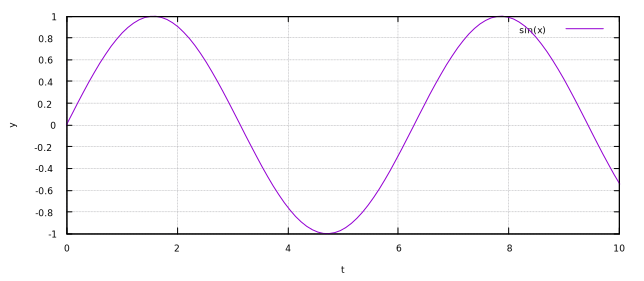
\includegraphics[width=0.9\textwidth]{Pictures/schwingung}

	\caption{Diagramm einer Schwingung: Elongation über der Zeit}

	
\end{figure}

\subsection{Kenngrößen von Schwingungen} \label{subsec:kenngroessen_schwingungen}


\subsubsection[Amplitude]{Amplitude: $y_{max}$ o. $s_{max}$ o. $\hat{y}$ o. $\hat{s}$ (Basiseinheit: $m$)}

Die maximale Elongation (=\glqq Auslenkung\grqq) der Schwingung.


\subsubsection[Periodendauer]{Periodendauer: $T$ (Basiseinheit: $s$)}
	
Die Zeit, die es dauert bis der schwindende Körper an der selben Stelle von der selben Richtung aus angelangt ist. Beispielsweise vom positiven Schwingungsmaximum (\glqq Berg\grqq) zum nächsten oder von der Nullstelle (\glqq Ruhelage\grqq) zur 2. darauffolgenden Nullstelle.

Davon abgeleitet:
\begin{itemize}
	\item Frequenz: $f=\frac{1}{T}$ (Basiseinheit: $Hz=\frac{1}{s}$)
	
	Anzahl der Perioden pro Sekunde.
	\item Winkelgeschwindigkeit: $\omega=2 \pi f=\frac{2 \pi}{T}$ (Basiseinheit: $\frac{rad}{s}$)
		
	Änderung des Winkels über der Zeit, wobei eine ganze Periode mit $360 \degree$ im Grad oder, im Physikunterricht verwendet, mit $2 \pi$ im Bogenmaß (eng: \glqq Radian\grqq) bezeichnet wird.\footnote{Umrechnung des Winkels $\alpha$ von Grad nach Bogenmaß: $\alpha_{rad} = \alpha_{deg} \cdot \frac{2\pi}{360 \degree} = \alpha_{deg} \cdot \frac{\pi}{180 \degree} $}
\end{itemize}


\subsubsection[Phasenverschiebung]{Phasenverschiebung: $\phi$ (Basiseinheit: $rad$)}
	
Wenn sich der Schwingungskörper zum Startzeitpunkt $t=0$ nicht in der Ruhelage $y=0$ befindet muss die Phasenverschiebung, z.B. zur Aufstellung der Schwingungsgleichung (\referenz{subsec:schwingungsgleichungen}), berücksichtigt werden. Die Phasenverschiebung gibt den Abstand von der y-Achse zum nächsten Durchlauf der Ruhelage von der negativen Seite.

	\begin{wrapfigure}{r}{0.5\textwidth} \label{phasenverschiebung}
	
		\vspace{-10pt}
		\includegraphics[width=0.48\textwidth]{Pictures/phasenverschiebung}
		\vspace{-13pt}
		\caption{Phasenverschiebung um $+\frac{3\pi}{2}$}
		\vspace{-5pt}
	
	\end{wrapfigure}

Im nebenstehenden Diagramm beträgt die Phasenverschiebung $\phi = +\frac{3\pi}{2}$, also ein Drei-Viertel der Periode. Man könnte ebenfalls sagen, die Phasenverschiebung beträgt $\phi = -\frac{\pi}{2}$, also minus Ein-Viertel der Periode. Beides ist äquivalent, jedoch ist es leichter mit einer positiven Phasenverschiebung zu rechnen.
	
	


\subsection{Schwingungsgleichungen} \label{subsec:schwingungsgleichungen}

Daraus ergibt sich folgende Schwingungsgleichung, bzw. Schwingungsfunktion, für eine harmonische Schwingung (\referenz{sec:definitionen}), die die Elongation in Abhängigkeit der Zeit angibt:

\begin{equation} \label{eq:schwingungsgleichung_y}
	y(t)=y_{max} \cdot \sin{(\omega t + \phi)}
\end{equation}

Die erste Ableitung dieser Gleichung nach $t$ gibt die Geschwindigkeit des Schwing-körpers zur Zeit $t$ an:

\begin{equation} \label{eq:schwingungsgleichung_v}
	y'(t)=v(t)=y_{max} \cdot \omega \cdot \cos{(\omega t + \phi)}
\end{equation}

Die zweite Ableitung gibt die Beschleunigung des Schwingkörpers zur Zeit $t$ an:

\begin{equation} \label{eq:schwingungsgleichung_a}
	y''(t)=v'(t)=a(t)=y_{max} \cdot \omega^{2} \cdot -\sin{(\omega t + \phi)}
\end{equation}


\subsection{Weitere Gleichungen und Gesetze}

\subsubsection{Gesetze im Kreis}

\paragraph{Bahngeschwindigkeit im Kreis}

Die Bahngeschwindigkeit gibt in absoluten Einheiten ($\frac{m}{s}$) an, wie schnell sich das Objekt auf der Bahn fortbewegt. Zusätzlich zur Winkelgeschwindigkeit (\referenz{subsec:kenngroessen_schwingungen}) muss bei der Kreisbahn daher noch der Radius bekannt sein:

\begin{equation*} \label{eq:bahngeschwindigkeit}
	v=\frac{2r\pi}{T}=\omega r
\end{equation*}

Eine andere Herleitung aus dem Kreisumfang $U=2r\pi$, der Periodendauer $T$ und der generellen Formel für Bahngeschwindigkeit $v=\frac{s(t)}{t}$ könnte wie folgt Aussehen:

\begin{align*}
	v&=\frac{s(t)}{t} \\
	v&=\frac{2r\pi}{T}
\end{align*}


\paragraph{Zentripetalbeschleunigung}

Um auf einer Kreisbahn zu bleiben, muss eine Zentripedalbeschleunigung auf einen Körper wirken, die zum Kreiszentrum hin zeigt. Die Formel lautet:

\begin{equation*}
	a_z=\frac{v^2}{r}=\omega^2 r
\end{equation*}


\paragraph{Zentripetalkraft}

Dies ist die Kraft, die auf einen Körper ausgewirkt werden muss, damit er auf einer Kreisbahn bleibt. Zusätzlich zur Zentripetalbeschleunigung muss nun also noch gemäß Newtons zweiten Axiom $F=a \cdot m$ die Masse als Faktor in die Gleichung aufgenommen werden:

\begin{align*}
	F_z &= a_z \cdot m \\
	F_z &= \frac{v^{2}m}{r}
\end{align*}


\subsubsection{Gesetze bei Geschwindigkeiten}

Aus der maximalen Geschwindigkeit und der Frequenz, Periodendauer oder Winkelgeschwindigkeit lässt sich sofort auf die Amplitude schließen, da in der Funktion für die Geschwindigkeit bei einer Schwingung (\referenz{subsec:schwingungsgleichungen}) $v(t)=\omega \cdot y_{max} \cdot \cos{(\omega t)}$ das Maxima dann erreicht ist, wenn der Cosinus seinen Maximalwert $1$ annimmt. Dann gilt folgendes:

\begin{align*} \label{eq:geschwindigkeit_amplitude}
	v_{max} &= \omega \cdot y_{max} \\
	v_{max} &= 2\pi f \cdot y_{max} \\
	y_{max} &= \frac{v_{max}}{2\pi f}
\end{align*}


\subsubsection{Gesetze am Federpendel}

\paragraph{Hooke'sches Gesetz}

Das Hooke'sche Gesetz gibt die Federhärte einer Feder, also dessen Kenngröße, an. Die Einheit $\frac{N}{m}$ erklärt selbst die Formel:

\begin{equation*}
	D=\frac{F}{l}
\end{equation*}

Mit dem Gesetz ist gezeigt, dass an einem Federpendel die Rückstellkraft $F$ proportional zur Auslenkung $l$ ist. Damit ist es eine harmonische Schwingung. (\referenz{subsec:definitionenzuschwingungen})

\paragraph{Periodendauer beim Federpendel}

Die Periodendauer beim Federpendel ist abhängig von der Masse $m$ und der Federkonstante $D$:

\begin{equation*}
	T_{Feder}=2\pi \cdot \frac{m}{D}
\end{equation*}

Die Herleitung gestaltet sich folgendermaßen: Die zur Auslenkung $y$ proportionale Kraft $F$ ist die Rückstellende Kraft; beschrieben durch eine Umformung des Hooke'schen Gesetzes: $F_{r}=D \cdot y$. 
%Der Vektor dieser Rückstellende Kraft zeigt dem der Auslenkenden Kraft genau entgegen, daher muss der Term in diesem Fall negiert werden: $F_{r}=-D \cdot y$.

In einem geschlossenen System ist die Summe aller Kräfte $0$. Es ergibt sich Folgendes:

\begin{align*}
	F_a + F_r &= 0 \\
	F_a &= -F_r \\
\end{align*}

Die Kraft $F_a$ kann wie jede Kraft mit Newtons zweitem Gesetz als $F_a=m \cdot a$ beschrieben werden. Die Beschleunigung in $a$ kann dann als zweite Ableitung der Auslenkung $y$ nach der Zeit beschrieben werden. Aus den Schwingungsgleichungen (\referenz{subsec:schwingungsgleichungen}) geht hervor, dass $y''=-\omega^{2} \cdot y$ ist. Daher kann man wie folgt einsetzen:

\begin{align*}
	m \cdot a &= -D \cdot y \\
	m \cdot y'' &= -D \cdot y \\
	m \cdot -\omega^{2} \cdot y &= -D \cdot y \\
	- m \cdot \omega^{2} &= -D \\
	\omega &= \sqrt{\frac{D}{m}}
\end{align*}

Für aus $\omega=\frac{2\pi}{T}$ folgt für $T$:

\begin{equation*}
	T = 2\pi \cdot \sqrt{\frac{m}{D}}
\end{equation*}














\section{Wellen -- Mathematisierung} \label{sec:wellen}
%%%%% Physik Kompendikum -- Wellen und Optik %%%%%
%% 03 Wellen %%


%Some sample text to be displayed above the first subsection

%\subsection{Prinzip}

%Ein Zyklotron besteht aus Zwei hohlen, halbzylindrischen und Duanden an denen eine Spannung mit unterschiedlichem Vorzeichen anliegt, und darüber bzw. darunter liegende Magneten, die ein homogenes Magnetfeld erzeugen. Zudem gibt es einen Einlass und einen Auslass für Teilchen.

%\begin{wrapfigure}{r}{0.4\textwidth} \label{Zyklo}
%
%	\vspace{-10pt}
%	\includegraphics[width=0.35\textwidth]{Zyklotron_Prinzipskizze02.png}
%	\vspace{-13pt}
%	\caption{Prinzipskizze eines Zyklotrons}
%	\vspace{-5pt}	
%	
%\end{wrapfigure}

%\subsubsection{Anwendung}

% Some Formula:

%\begin{equation}
%	x= \frac{y \cdot 13 \pi z}
%			{\cos \alpha}
%\end{equation}

%%%%%%%%%%%%%%%%%%%%%%%
% Eigentlicher Beginn %
%%%%%%%%%%%%%%%%%%%%%%%

\subsection{Diagramme von Wellen} \label{subsec:diagramm_welle}

Einer Welle reicht ein Diagramm zur Darstellung nicht aus. Da es sehr viele Oszillatoren gibt, die alle zu unterschiedlichen Zeiten zu schwingen beginnen, bräuchte man ein Elongation-Zeit-Diagramm (\referenz{subsec:diagramm_schwingung}) für jedes Teilchen, oder ein 3-dimensionales Diagramm.

Allerdings reichen zwei Diagramme, davon ein Elongation-Zeit-Diagramm eines beliebigen Teilchens und ein Elongation-Strecke-Diagramm (auch bekannt als \glqq Standbild\grqq) zu einem beliebigen Zeitpunkt, um alle Kenngrößen der Welle erfassen zu können.



\subsection{Kenngrößen}


\subsubsection[Amplitude]{Amplitude: $y_{max}$ o. $s_{max}$ o. $\hat{y}$ o. $\hat{s}$ (Basiseinheit: $m$)}

\textbf{Kategorie: Schwingung \textit{eines} Oszillators}

Die maximale Elongation (=\glqq Auslenkung\grqq) der Schwingungen der einzelnen Oszillatoren.



\subsubsection[Periodendauer]{Periodendauer: $T$ (Basiseinheit: $s$)}

\textbf{Kategorie: Schwingung \textit{eines} Oszillators}
	
Die Zeit, die es dauert bis einer der schwindenden Körper an der selben Stelle von der selben Richtung aus angelangt ist. Beispielsweise vom positiven Schwingungsmaximum (\glqq Berg\grqq) zum nächsten oder von der Nullstelle (\glqq Ruhelage\grqq) zur 2. darauffolgenden Nullstelle.

Davon abgeleitet:
\begin{itemize}
	\item Frequenz: $f=\frac{1}{T}$ (Basiseinheit: $Hz=\frac{1}{s}$)
	
	Anzahl der Perioden pro Sekunde.
	\item Winkelgeschwindigkeit: $\omega=2 \pi f=\frac{2 \pi}{T}$ (Basiseinheit: $\frac{rad}{s}$)
		
	Änderung des Winkels über der Zeit, wobei eine ganze Periode mit $360 \degree$ im Grad oder, im Physikunterricht verwendet, mit $2 \pi$ im Bogenmaß (eng: \glqq Radian\grqq) bezeichnet wird.\footnote{Umrechnung des Winkels $\alpha$ von Grad nach Bogenmaß: $\alpha_{rad} = \alpha_{deg} \cdot \frac{2\pi}{360 \degree} = \alpha_{deg} \cdot \frac{\pi}{180 \degree} $}
\end{itemize}



\subsubsection[Wellenlänge]{Wellenlänge: $\lambda$ (Basiseinheit: $m$)}

\textbf{Kategorie: Oszillatorsystem}

Der räumliche Abstand zwischen 2 Wellenbergen im Elongation-Strecke-Diagramm, der Abstand eines Nulldurchlaufs mit dem zweiten darauffolgenden.



\subsubsection[Ausbreitungsgeschwindigkeit]{Ausbreitungsgeschwindigkeit: $c$ (Basiseinheit: $\frac{m}{s}$)}

Die Ausbreitungsgeschwindigkeit ist eigentlich keine echte Kenngröße, da sie nicht in der Wellengleichung auftaucht. Trotzdem ist sie hilfreich um $\lambda$ oder $f$ zu berechnen. Die Gleichung lautet:

\begin{equation} \label{eq:wellen_c}
	c=\lambda \cdot f=\frac{\lambda}{T}
\end{equation}



\subsection{Wellengleichungen}

Die Wellengleichung gibt die Elongation des Teilchens mit dem Abstand $x$ zum Ausgangspunkt zum Zeitpunkt $t$ an:

\begin{equation} \label{eq:wellengleichung_y}
	y(x,t) = y_{max} \cdot sin{ (2\pi(\frac{t}{T}-\frac{x}{\lambda})) }
\end{equation}

Zur Herleitung aus der Schwingungsgleichung muss Folgendes beachtet werden. Die Zeit $t_x$ bis das räumliche Teilchen $x$ von der Front der Welle erfasst wird, lässt sich recht einfach berechnen. Gebraucht wird dabei die Ausbreitungsgeschwindigkeit $c=\frac{\lambda}{T}$ die generelle Formulierung der Geschwindigkeit $v=\frac{s}{t}$:

\begin{align*}
	t   &= \frac{s}{v} \\
	t_x &= \frac{x}{c} \\
	t_x &= \frac{x \cdot T}{\lambda}
\end{align*}

Analog zur Verschiebung nach rechts von beispielsweise einer Parabel, muss der Term für $t_x$ von $t$ in der Schwingungsgleichung abgezogen werden. Damit ist die Variable $x$ mit in der Gleichung und der Term \glqq kompensiert\grqq{} den \glqq Offset\grqq{}, der sich durch das spätere Erfassen ergibt:

\begin{align*}
	y(x,t) &= y_{max} \cdot sin{[\omega \cdot (t-\frac{x}{\lambda} \cdot T)]} \\
	y(x,t) &= y_{max} \cdot sin{[\frac{2\pi}{T} \cdot (t-\frac{x}{\lambda} \cdot T)]} \\
	y(x,t) &= y_{max} \cdot sin{[2\pi \cdot (\frac{t}{T}-\frac{x}{\lambda \cdot T} \cdot T)]} \\
	y(x,t) &= y_{max} \cdot sin{[2\pi \cdot (\frac{t}{T}-\frac{x}{\lambda})]}
\end{align*}



\subsection{Weitere Gleichungen und Gesetze}

\subsubsection{Wellenfront}

\paragraph{Erreichen eines beliebigen Teilchens}

Analog zu $v=\frac{s}{t}$:

\begin{equation*}
	t=\frac{x}{\lambda}
\end{equation*}















\section{Wellen -- Eigenschaften und Phänomene} \label{sec:wellen_eigenschaften}
%%%%% Kompendium -- Wellen und Optik %%%%%
%% Wellen -- Eigenschaften und Phänomene %%


%Some sample text to be displayed above the first subsection

%\subsection{Prinzip}

%Ein Zyklotron besteht aus Zwei hohlen, halbzylindrischen und Duanden an denen eine Spannung mit unterschiedlichem Vorzeichen anliegt, und darüber bzw. darunter liegende Magneten, die ein homogenes Magnetfeld erzeugen. Zudem gibt es einen Einlass und einen Auslass für Teilchen.

%\begin{wrapfigure}{r}{0.4\textwidth} \label{Zyklo}
%
%	\vspace{-10pt}
%	\includegraphics[width=0.35\textwidth]{Zyklotron_Prinzipskizze02.png}
%	\vspace{-13pt}
%	\caption{Prinzipskizze eines Zyklotrons}
%	\vspace{-5pt}	
%	
%\end{wrapfigure}

%\subsubsection{Anwendung}

% Some Formula:

%\begin{equation}
%	x= \frac{y \cdot 13 \pi z}
%			{\cos \alpha}
%\end{equation}

%%%%%%%%%%%%%%%%%%%%%%%
% Eigentlicher Beginn %
%%%%%%%%%%%%%%%%%%%%%%%

Im Folgenden werden bei der Nennung von \glqq Wellen\grqq{} immer Transversalwellen gemeint, wenn es keine weitere Anmerkung gibt.  



\subsection{Reflexion}  

	\paragraph{Fixiertes Ende}
	
	Wenn eine Welle von einem fixierten Ende (eingespannt) reflektiert wird, dann gibt es einen Phasensprung von $180 \degree$ oder $\pi$, bzw $\frac{T}{2}$.
	
	\paragraph{Loses Ende}
	
	Trifft eine Welle auf ein loses Ende, dann wird sie ohne  Phasensprung reflektiert.



\subsection{Überlagerung}

Wenn sich Wellen in einem räumlichen Punkt treffen, dann überlagern sie sich und bilden eine summierte Welle. Wenn also ein Wellenberg auf einen Wellenberg trifft, addieren sich beide Welle und der resultierende Wellenberg ist höher. Sollte auf einen Wellenberg ein Wellental treffen wird auf addiert, und die resultierende Welle von der Amplitude her kleiner.

Nachdem sich die Wellen in diesem Punkt überlagert haben, laufen beide weiter ohne die andere zu beeinflussen; so als hätte es die Überlagerung nie gegeben.

	\subsubsection{Stehende Welle}
	
	Wenn sich gegenläufige, das heißt parallel und identisch, aber in die entgegengesetzte Richtung fortschreitende, Wellen mit derselben Wellenlänge überlagern, entsteht eine stehende Welle. 
	Das heißt, dass es mindestens 2 Oszillatoren auf dieser Welle gibt, die sich gar nicht bewegen (\glqq stehen\grqq), die sogenannten Knotenpunkte.
	
	Eine stehende Welle kann zum Beispiel ausgelöst werden, wenn bei einer Reflexion am festen Ende die Hälfte der Wellenlänge $\lambda$ ein ganzzahliges Vielfaches der Abstands $l$ der beiden Enden ist. $k$ ist in diesem Fall eine Variable, die nur positive ganze Zahlen annehmen kann:
	
	\begin{equation} \label{stehendewelle}
		\lambda = 2k \cdot l \ \ \ wobei \ \ k \in 1,2,3...
	\end{equation}



\subsection{Interferenzen} \label{sec:interferenz}

Wenn sich Wellen, die nicht nur dieselbe Wellenlänge, sondern auch die selbe Amplitude aufweisen, in einem Punkt überlagern, dann kann es zu Interferenzen kommen.

	\subsubsection{Konstruktive Interferenz}
	
	Wenn in dem Punkt beide Wellen ein Maximum aufweisen, sich also zu einem höheren Wellenberg addieren, spricht man von konstruktiver Interferenz.
	
	Dazu muss der Gangunterschied $\delta$ ein ganzzahliges Vielfaches der Wellenlänge sein:
	
	\begin{equation}	\label{eq:kon_interferenz}
		\delta = k \cdot \lambda \ \ \ wobei \ \ k \in 1,2,3...
	\end{equation}
	
	\subsubsection{Destruktive Interferenz}
	
	Im Gegensatz zur konstruktiven Interferenz, treffen nun also Wellen aufeinander, die einmal einen Wellenberg und einmal ein Wellental aufweisen. Da sie dieselbe Amplitude haben, ist die resultierende Amplitude im betroffenen Punkt $0$.
	
	Der Gangunterschied $\delta$ muss daher die Summe eines ganzzahliges Vielfaches Wellenlänge und der halben Wellenlänge sein:
	
	\begin{equation}
		\delta = k \cdot \lambda + \frac{\lambda}{2} \ \ \ wobei \ \ k \in 1,2,3...
	\end{equation}

	Zur einfacheren Umstellung nach $\lambda$ existiert diese, internationale Form:
	
	\begin{equation} \label{eq:des_interferenz}
		\delta = (2k -1) \cdot \frac{\lambda}{2} \ \ \ wobei \ \ k \in 1,2,3...
	\end{equation}



\subsection[Ausbreitung in Elementarwellen]{Ausbreitung in Elementarwellen (Huygens'sches Prinzip)} \label{subsec:ausbreitung}

Das Huygens'sche Prinzip macht eine wichtige Aussage zur Ausbreitung von Wellen:

\glqq Jedes Teilchen (Oszillator), das von einer Wellenfront erfasst wird, löst von sich aus eine zirkulare Welle nach allen Seiten aus.\grqq{} Die eigentlich sichtbare Wellenfront ist nach Huygens eine Einhüllende aller \glqq Elementarwellen\grqq . Dadurch ist es Wellen unter anderem möglich in den geometrischen Schattenraum zu propagieren. \referenz{subsec:doppelspalt}


\subsection{Wellen am Doppelspalt} \label{subsec:doppelspalt}

Wenn nun eine räumlich und zeitlich kohärente Wellen, das heißt Wellenfronten deren Wellen sowohl parallel als auch phasengleich (mit derselben Wellenlänge und Gangunterschied $\delta= k \cdot \lambda$) verlaufen, auf ein Hindernis mit 2 schmalen Spalten trifft, bildet sich folgendes Interferenzmuster:

%\begin{figure}[h!]
%	\center
%	\includegraphics[width=0.4\textwidth]{doppelspalt_wasser}
%	\caption{Eine kohärente Welle am Doppelspalt}
%\end{figure}

Dies ist mit dem Huygens'schen Prinzip (\referenz{subsec:ausbreitung}) zu erklären: Angenommen, in jedem Spalt gäbe es nur ein schwingendes Teilchen. Dieses wird von der Wellenfront erfasst und ist selber Auslöser einer zirkularen Wellen. Da dieser Oszillator an dieser Stelle der einzige ist, gibt es keine gerade Wellenfront als Einhüllende, sondern einzig die Zirkularwelle des angeregten Oszillators.


\subsubsection{Mathematisierung}

	Der Versuch ist auch mit Laserlicht, also Monochromatisch (eine einzige Wellenlänge) und Kohärent, durchführbar. Das Licht wird durch einen schmalen Doppelspalt mit dem Spaltabstand $d \leq 2mm$ hinter dem sich im Abstand $a$ ein Schirm befindet. 
	
	Auf dem Schirm ist ein Interferenzmuster zu beobachten. In der Mitte ist ein heller Streifen, links und rechts davon, symmetrisch, sind weniger intensive Lichtpunkte. Diese Punkte werden Maxima genannt, da in diesen Punkten konstruktive Interferenz herrscht (\referenz{sec:interferenz}). An den Minimalstellen herrschen destruktive Interferenzen. Der Gangunterschied ergibt sich hier durch den Unterschiedlichen Abstand der Punkte auf dem Schirm zu dem beiden Schlitzen.
	
	Eine Zeichnung:
	
%	\begin{figure}[h!]
%		\center
%		\includegraphics[width=0.8\textwidth]{default}
%		\caption{Das Maxima 1. Ordnung am Doppelspalt}
%	\end{figure}
	
	Die Winkel $\alpha_a$ und $\alpha_d$ sind gleich und werden im Folgen schlicht als $\alpha$ bezeichnet. Für $\alpha$ ergeben sich aus den trigonomischen Winkelfunktionen im rechtwinkligen Dreieck 2 Gleichungen: $sin{\alpha}=\frac{\delta}{d}$ und $tan{\alpha}=\frac{d_k}{a}$. Da $a>>d_k$ ist $\alpha<10 \degree$ und die Kleinwinkelnäherung $sin{\alpha} \approx \tan{alpha}$ kann verwendet werden. Der Gangunterschied $\delta$ muss der Bedingung für konstruktive Interferenz $\delta = k \cdot \lambda$ genügen (Siehe Gleichung \ref{eq:kon_interferenz} auf Seite \pageref{eq:kon_interferenz}). Daraus Ergibt sich:
	
	\begin{align}
		\sin{\alpha} &= \tan{\alpha} \\
		\frac{\delta}{d} &= \frac{d_k}{a} \\
		\frac{k \cdot \lambda}{d} &= \frac{d_k}{a}  \ \ \ wobei \ \ k \in 1,2,3... \\
		\lambda &= \frac{d_{k} \cdot d}{a \cdot k}  \ \ \ wobei \ \ k \in 1,2,3...
	\end{align}
	
	Für $k$ muss die Ordnung des betrachteten Maxima eingesetzt werden.
		

\subsubsection{Ohne Kleinwinkelnäherung}

	Um präziser ablesen zu können, kann ein Gitter statt einem Doppelspalt verwendet werden. Das Gitter weist einen wesentlich geringeren Abstand zwischen den Schlitzen auf (z.B. $\frac{1}{600}mm$), sodass die Interferenzmaxima deutlich weiter auseinander liegen. Der Fakt, dass der Lichtdurchsatz durch das Hinzufügen von mehr Schlitzen zu einem Gitter erhöht wurde, ändert nichts an den mathematischen Grundlagen des Versuchs.
	
	Allerdings geht mit dem größeren Abstand der Punkte auf dem Schirm die Gültigkeit der Kleinwinkelnäherung verloren. Allerdings kann die Größe des Winkels $\alpha_a$ über $\arctan{\frac{d_k}{a}}$ berechnet werden und in die Gleichung $\sin{\alpha} = \frac{\delta}{d}$ eingesetzt werden:
	
	\begin{align}
		\frac{\delta}{d} &= \sin{\alpha} \\
		 \delta &= \sin{(\arctan{\frac{d_k}{a}})} \cdot d \\
		\lambda \cdot k &= \sin{(\arctan{\frac{d_k}{a}})} \cdot d \ \ \ wobei \ \ k \in 1,2,3... \\
		\lambda &= \frac{\sin{(\arctan{\frac{d_k}{a}})} \cdot d}{k} \ \ \ wobei \ \ k \in 1,2,3...
	\end{align}


\subsection{Lichtspektrum am Doppelspalt}

Wenn ein Lichtspektrum (z.B. weißes Licht von einer Glühbirne) auf einen Doppelspalt oder ein Gitter trifft, dann tritt dasselbe Phänomen wie bei monochromatischem Licht, mit dem Unterschied, dass die unterschiedlichen Wellenlängen im Spektrum ihren eigenen, von der Wellenlänge abhängigen, Abstand $d_k$ haben. Dadurch wird das Lichtspektrum von violett bis rot aufgefächert (Dispersion).













\section{Elektromagnetische Wellen} \label{sec:em_wellen}
%%%%% TITLE OF MAIN DOCUMENT %%%%%
%% NUMBER AND TITLE OF SECTION %%


%Some sample text to be displayed above the first subsection

%\subsection{Prinzip}

%Ein Zyklotron besteht aus Zwei hohlen, halbzylindrischen und Duanden an denen eine Spannung mit unterschiedlichem Vorzeichen anliegt, und darüber bzw. darunter liegende Magneten, die ein homogenes Magnetfeld erzeugen. Zudem gibt es einen Einlass und einen Auslass für Teilchen.

%\begin{wrapfigure}{r}{0.4\textwidth} \label{Zyklo}
%
%	\vspace{-10pt}
%	\includegraphics[width=0.35\textwidth]{Zyklotron_Prinzipskizze02.png}
%	\vspace{-13pt}
%	\caption{Prinzipskizze eines Zyklotrons}
%	\vspace{-5pt}	
%	
%\end{wrapfigure}

%\subsubsection{Anwendung}

% Some Formula:

%\begin{equation}
%	x= \frac{y \cdot 13 \pi z}
%			{\cos \alpha}
%\end{equation}

%%%%%%%%%%%%%%%%%%%%%%%
% Eigentlicher Beginn %
%%%%%%%%%%%%%%%%%%%%%%%

Als elektromagnetische Wellen bezeichnet man alle Wellen, bei denen gekoppelten elektrischen und magnetische Felder schwingen. Die Schwingungsverktoren der beiden Felder stehen jeweils senkrecht aufeinander und senkrecht auf dem Vektor der Ausbreitungsrichtung:\footnote{„Onde electromagnetique“ von SuperManu - Self, based on Image:Onde electromagnetique.png. Lizenziert unter CC BY-SA 3.0 über Wikimedia Commons - \url{https://commons.wikimedia.org/wiki/File:Onde_electromagnetique.svg}}

\begin{figure}[h!]
	\center
	\includegraphics[width=0.8\textwidth]{em_welle}
	\caption{Eine elektromagnetische Welle}
\end{figure}

Im Vakuum bzw. in der Luft bewegen sich alle elektromagnetischen Wellen mit Lichtgeschwindigkeit fort. (Taschenrechner: Konstante 28: $c_0=299.792.458 \frac{m}{s}$)

\subsection{Spektrum}
\hspace{-60pt}
\begin{tabular}[c]{|c|c|c|l|}
	\hline
	Name				&	$f$						& $\lambda$ 	& Kommentar\\
	\hline
	Längstwellen		&	$15-200Hz$				& $10^6-10^7m$ & Strom; Nur Nahfeld\\
	Radiowellen			&	$10^4-10^8Hz$			& $10^0-10^4m$ & \\
	Mikrowellen			&	$10^8-10^{11}Hz$		& $10^{-3}-10^{0}m$ & \\
	Infrarotes Licht	&	$>10^{12}Hz$			& $<10^{-4}m$ & \glqq Wäremestrahlung\grqq \\
	Sichtbares Licht	&	$\approx 10^{15}Hz$		& $400-800nm$ $\approx 10^{-6}m$ & sichtbar\\
	Röntgenstrahlung	&	$10^{16} - 10^{20}Hz$	& $10^{-12}-10^{-8}m$ & Erzeugung: schnelle $e^{-}$ auf Metall \\
	Gammastrahlung		&	$>10^{20}Hz$			& $<10^{-12}m$ & \\
	\hline
\end{tabular}













\section{Optik} \label{sec:optik}
\input{KompendiumSchwingungen/Chapters/optik}




\chapter{Quanten}
\input{KompendiumQuanten/Quanten}

\addtocontents{toc}{\protect\setcounter{tocdepth}{1}}
\appendix

	\chapter{Beispielaufgabe -- Optik}
	\section*{Aufgabenstellung}

Die Brechzahl in einer bestimmten Glassorte beträgt für rotes Licht $n_{rot} = 1,51$ und für blaues Licht $n_{blau} = 1,52$. Auf ein Prisma, dessen Querschnittsfläche ein gleichseitiges Dreieck ist, fällt ein schmales Lichtbündel mit einem Einfallswinkel von $45 \degree$. Das Licht wird auf einem $2m$ entfernten Schirm aufgefangen. Berechnen Sie den Abstand des blauen und des roten Bereichs im Spektrum auf dem Schirm.



\section{Annahmen}

\subsection{Schirm}

Der Schirm sei gerade und weise gleiche Winkel zu den beiden äußersten Strahlen des Spektrums auf.

\section{Prisma}

Das Prisma sei so klein, dass der Unterschied der Austrittspunkte für die Strahlen unterschiedlicher Wellenlängen vernachlässigt werden können und Punkt S als uniformer Austrittspunkt der Strahlen aus dem Prisma. Die Winkel mit welchen das Licht auf den Punkt S auftrifft, werden jedoch berücksichtigt, da diese unabhängig von der Größe des Prismas sind.

\section{Zeichnung}	\label{sec:zeichnung}

\begin{figure}[ht!]
	\vspace{-15px}	
	\begin{center}
		\includegraphics[width=0.9\textwidth]{skizze}
		\caption{Zeichnung}
	\end{center}	
\end{figure}

\section{Angaben} \label{sec:Angaben}

\subsection{Geometrie}

\begin{multicols}{2}
	\noindent
	\begin{align*}
		\epsilon      &= 360 \degree - 60 \degree - 2 \cdot 90 \degree = 120 \degree \\
		\delta_{rot}  &= \delta_{blau} \\
		\overline{BR} &= 2 \cdot \overline{BP}
	\end{align*}
\end{multicols}

\subsection{Aufgabenstellung}

\begin{multicols}{3}
	\noindent
	\begin{align*}
		n_{rot}       &= 1,51 \\
		n_{blau}      &= 1,52
	\end{align*}
	\begin{align*}
		\alpha_{1}    &= 45 \degree \\
		\overline{SP} &= 2m
	\end{align*}
\end{multicols}


\section{Gesetze}

\subsection{Brechungsgesetz}

\begin{equation}
\frac{\sin{(\alpha)}}{\sin{(\beta})} = \frac{n_{2}}{n_{1}} \ <=> \ 
\sin{(\beta)} = \frac{sin{(\alpha)} \cdot n_{1}}{n_{2}} \label{eq:brechung}
\end{equation}


\section{Berechnung}



\subsection{Rotes Licht -- Eintritt in Prisma}

$n_1 = 1$ \ \ \ \ ; da Luft o. Vakuum \\
$n_2 = 1,51$     ; da rotes Licht


\begin{align*}
	sin{(\beta_{1,rot})} &= \frac{sin{(\alpha})}{n_2} \\
	sin{(\beta_{1,rot})} &= \frac{sin{(45 \degree})}{1,51} \approx 0,46828 \\
	\beta_{1,rot} &= \arcsin{(0,46828)} \approx 27,92288 \degree \approx 27,923 \degree
\end{align*}



\subsection{Rotes Licht -- Austritt in Prisma}

Der neue Einfallswinkel $\alpha_{2,rot}$ lässt sich direkt aus $\beta_{1,rot}$ und den Winkeleigenschaften des gleichseitigen Dreiecks berechnen. (siehe Sektion \ref{sec:Angaben} \ auf Seite \pageref{sec:Angaben})
\begin{align*}
	\alpha_{2,rot} &= 180 \degree - \epsilon - \beta_{1,rot} \\
	\alpha_{2,rot} &= 180 \degree - 120 \degree - 27,92288 \degree = 32,07712 \degree
\end{align*}

\noindent
$n_1 = 1,51$     ; da rotes Licht \\
$n_2 = 1$ \ \ \ \ ; da Luft o. Vakuum

\begin{align*}
	sin{(\beta_{2,rot})} &= \frac{sin{(\alpha_{2,rot}})}{n_2} \\
	sin{(\beta_{2,rot})} &= \frac{sin{(32,07712 \degree})}{1,51} \approx 0,8019 \\
	\beta_{2,rot} &= \arcsin{(0,8019)} \approx 53,312 \degree
\end{align*}



\subsection{Blaues Licht -- Eintritt in Prisma}

$n_1 = 1$ \ \ \ \ ; da Luft o. Vakuum \\
$n_2 = 1,52$     ; da blaues Licht


\begin{align*}
	sin{(\beta_{1,blau})} &= \frac{sin{(\alpha_{1}})}{n_2} \\
	sin{(\beta_{1,blau})} &= \frac{sin{(45 \degree})}{1,52} \approx 0,465202 \\
	\beta_{1,blau} &= \arcsin{(0,465202)} \approx 27,723
\end{align*}



\subsection{Blaues Licht -- Austritt in Prisma}

Auch der neue Einfallswinkel $\alpha_{2,blau}$ lässt sich direkt aus $\beta_{1,blau}$ und den Winkeleigenschaften des gleichseitigen Dreiecks berechnen. (siehe Sektion \ref{sec:Angaben} \ auf Seite \pageref{sec:Angaben})
\begin{align*}
	\alpha_{2,blau} &= 180 \degree - \epsilon - \beta_{1,blau} \\
	\alpha_{2,blau} &= 180 \degree - 120 \degree - 27,723 \degree = 32,277 \degree
\end{align*}

\noindent
$n_1 = 1,52$     ; da blaues Licht \\
$n_2 = 1$ \ \ \ \ ; da Luft o. Vakuum

\begin{align*}
	sin{(\beta_{2,blau})} &= \frac{sin{(\alpha_{2,blau}})}{n_2} \\
	sin{(\beta_{2,blau})} &= \frac{sin{(32,277 \degree})}{1,52} \approx 0,8116 \\
	\beta_{2,rot} &= \arcsin{(0,8116)} \approx 54,253 \degree
\end{align*}



\subsection{Spektrum -- Abstand auf Schirm}

Der Winkel $\delta$ (Siehe Sektion \ref{sec:zeichnung} auf Seite \pageref{sec:zeichnung}) ist die Different der beiden Austrittswinkel $\beta_{2,blau}$ und $\beta_{2,rot}$.

\begin{equation}
	\delta = \beta_{2,blau} - \beta_{2,rot} = 54,253 \degree - 53,312 \degree = 0,941 \degree
\end{equation}

Der Tangenz von $\frac{\delta}{2}$ ist der Quotient der Hälfte der Strecke $RB$ als Gegenkathete und der Strecke $SP$ als Ankathete. Daraus ergibt sich folgendes für die Länge der Strecke $RB$:

\begin{align*}
\tan{(\frac{\delta}{2})} &= \frac{\frac{1}{2} \cdot \overline{RB}}{\overline{SP}}
    = \frac{\overline{RB}}{2 \cdot \overline{SP}}
	\ \ \ | \cdot 2 \ ; \ \cdot \overline{SP} \\
\overline{RB} &= 2 \tan{(\frac{\delta}{2})} \cdot \overline{SP} \\
\overline{RB} &= 2 \tan{(\frac{\delta}{2})} \cdot 2m \approx 0,03285m \ \widehat{=} \ 3,285cm
\end{align*}


\section{Antwort}

Der Abstand des roten und blauen Bereichs auf dem Schirm, also in etwa die Breite des aufgefächerten Spektrums, beträgt ca. $3,285cm$.




\end{document}
